\documentclass[12pt,a4paper]{article}

% ---- Encoding ----
\usepackage{multirow}
\usepackage[utf8]{inputenc}
\usepackage[T5]{fontenc}
\usepackage[vietnamese]{babel}

% ---- Math ----
\usepackage{amsmath}
\usepackage{amsfonts}

% ---- Graphics ----
\usepackage{graphicx}

% ---- Layout ----
\usepackage{geometry}
\geometry{a4paper, left=3cm, right=2cm, top=2.5cm, bottom=2.5cm}
\usepackage{setspace}
\setstretch{1.3}
\usepackage{indentfirst}
\setlength{\parindent}{1.2em}
\setlength{\parskip}{3pt}

% ---- Header / Footer ----
\usepackage{fancyhdr}
\usepackage{lastpage}
\pagestyle{fancy}
\fancyhf{}
\fancyfoot[R]{\small\thepage}
\renewcommand{\headrulewidth}{0pt}
\renewcommand{\footrulewidth}{0pt}

% ---- Tables ----
\usepackage{tabularx}
\usepackage{booktabs}
\usepackage{multirow}
\usepackage{float}

% ---- TOC Customization ----
\usepackage{tocloft}
% Title 'MỤC LỤC' centered, bold, uppercase
\renewcommand{\contentsname}{MỤC LỤC}
\renewcommand{\cfttoctitlefont}{\hfill\Large\bfseries}
\renewcommand{\cftaftertoctitle}{\hfill\null\par\vspace{0.5em}}
% List of Figures / Tables titles
\renewcommand{\listfigurename}{DANH MỤC HÌNH VẼ}
\renewcommand{\cftloftitlefont}{\hfill\Large\bfseries}
\renewcommand{\cftafterloftitle}{\hfill}
\renewcommand{\listtablename}{DANH MỤC BẢNG BIỂU}
\renewcommand{\cftlottitlefont}{\hfill\Large\bfseries}
\renewcommand{\cftafterlottitle}{\hfill}
% Section entries: bold text + bold page number
\renewcommand{\cftsecfont}{\bfseries}
\renewcommand{\cftsecpagefont}{\bfseries}
% Dots for sections too
\renewcommand{\cftsecleader}{\cftdotfill{\cftdotsep}}
% Extra vertical space before each section entry
\setlength{\cftbeforesecskip}{8pt}
% Normal spacing for subsections
\setlength{\cftbeforesubsecskip}{1pt}
% Indent adjustments
\setlength{\cftsecindent}{0pt}
\setlength{\cftsubsecindent}{1.5em}
\setlength{\cftsubsubsecindent}{3.5em}

% ---- Enable numbering & TOC entries down to \paragraph (X.Y.Z.W) and \subparagraph (A./B./C.) ----
\setcounter{secnumdepth}{5}
\setcounter{tocdepth}{5}
\makeatletter
\renewcommand{\l@paragraph}[2]{\@dottedtocline{4}{7.6em}{4.2em}{#1}{#2}}
\renewcommand{\l@subparagraph}[2]{\@dottedtocline{5}{9.8em}{3.0em}{#1}{#2}}
\makeatother
\renewcommand{\thesubparagraph}{\Alph{subparagraph}.}

% ---- Links ----
\usepackage[colorlinks=true, linkcolor=black, urlcolor=blue, citecolor=green!50!black]{hyperref}

% ---- Code Listings ----
\usepackage{listings}
\usepackage{xcolor}

% ---- Flowchart / Diagram (TikZ) ----
\usepackage{tikz}
\usetikzlibrary{shapes.geometric, arrows.meta, positioning, fit, calc}
\tikzset{
    startstop/.style={rectangle, rounded corners, minimum width=2.6cm, minimum height=0.9cm, text width=3cm, align=center, draw=black, fill=gray!15, font=\small},
    process/.style={rectangle, minimum width=3cm, minimum height=0.9cm, text width=3cm, align=center, draw=black, fill=blue!6, font=\small},
    decision/.style={diamond, aspect=2.2, minimum width=2.6cm, minimum height=1cm, text width=2cm, align=center, draw=black, fill=orange!12, font=\scriptsize, inner sep=1pt},
    ioblk/.style={trapezium, trapezium left angle=70, trapezium right angle=110, minimum width=2.6cm, minimum height=0.8cm, text width=3.2cm, align=center, draw=black, fill=green!8, font=\small},
    arrowline/.style={-{Latex[length=2mm]}, thick}
}

\definecolor{codegreen}{rgb}{0,0.6,0}
\definecolor{codegray}{rgb}{0.5,0.5,0.5}
\definecolor{codepurple}{rgb}{0.58,0,0.82}
\definecolor{backcolour}{rgb}{0.95,0.95,0.92}

\lstset{
    backgroundcolor=\color{backcolour},
    commentstyle=\color{codegreen},
    keywordstyle=\color{magenta},
    numberstyle=\tiny\color{codegray},
    stringstyle=\color{codepurple},
    basicstyle=\ttfamily\small,
    breakatwhitespace=false,
    breaklines=true,
    captionpos=b,
    keepspaces=true,
    numbers=left,
    numbersep=5pt,
    showspaces=false,
    showstringspaces=false,
    showtabs=false,
    tabsize=2
}

\begin{document}

% ============================================================
%  TRANG BÌA
% ============================================================
\begin{titlepage}
    \begin{center}
        \textbf{ĐẠI HỌC BÁCH KHOA HÀ NỘI}\\
        Trường Điện -- Điện tử
    \end{center}

    \vspace{1.2cm}
    \begin{figure}[h]
        \centering
        \includegraphics[width=0.35\textwidth]{images/logo.png}
    \end{figure}

    \vspace*{\fill}

    \begin{center}
        \textbf{\Large TRẠM QUAN TRẮC CHẤT LƯỢNG KHÔNG KHÍ ĐA THÔNG SỐ}\\[5pt]
        \large Kỹ thuật vi xử lý\\[10pt]
    \end{center}

    \hspace{1cm}\textbf{Nhóm 22 - Lớp 169227:}

    \begin{table}[h]
        \centering
        \begin{tabular}{|c|l|c|}
        \hline
            \textbf{STT} & \textbf{Họ và tên} & \textbf{MSSV}\\ 
        \hline
            1 & Tống Quang Giáp   & 20223947\\ 
        \hline
            2 & Nguyễn Danh Trung & 20224176\\ 
        \hline
            3 & Nguyễn Huy Hoàng  & 20223984\\ 
        \hline
        \end{tabular}
    \end{table}

    \hspace{1cm}\textbf{Giảng viên hướng dẫn:} TS. Hàn Huy Dũng\\

    \vspace*{\fill}

    \begin{center}
        Hà Nội -- \today
    \end{center}
\end{titlepage}

\newpage
\begin{center}
    \textbf{\Large LỜI CẢM ƠN}
\end{center}
\vspace{1cm}

Lời đầu tiên nhóm em xin chân thành cảm ơn Tiến sĩ Hàn Huy Dũng vì sự hướng dẫn tận tình, sự kiên nhẫn vô hạn và những đóng góp quý báu của thầy trong việc giúp đỡ nhóm em hoàn thành bài tập lớn này.

Nhóm em cũng xin nói lời cảm ơn đến tất cả các anh trợ giảng của thầy Dũng, đặc biệt là anh Hiếu và anh Sơn đã góp ý và đưa ra những nhận xét rất thiết thực cho nhóm em trong thời gian hoàn thiện bài tập lớn này.

\newpage
\begin{center}
    \textbf{\Large LỜI CAM ĐOAN}
\end{center}
\vspace{1cm}

Nhóm em là nhóm 22, bao gồm 3 thành viên Nguyễn Huy Hoàng, MSSV: 20223984; Nguyễn Danh Trung, MSSV: 20224176; Tống Quang Giáp, MSSV: 2022394. Người hướng dẫn là TS. Hàn Huy Dũng. Nhóm em xin cam đoan toàn bộ nội dung được trình bày trong dự án Trạm quan trắc chất lượng không khí đa thông số là kết quả quá trình tìm hiểu và nghiên cứu của nhóm. Các dữ liệu được nêu trong báo cáo là hoàn toàn trung thực, phản ánh đúng kết quả đo đạc thực tế. Mọi thông tin trích dẫn đều tuân thủ các quy định về sở hữu trí tuệ, các tài liệu tham khảo được liệt kê rõ ràng. Nhóm xin chịu hoàn toàn trách nhiệm với những nội dung được viết trong báo cáo này.

\vspace{1.5cm}
\begin{flushright}
Hà Nội, ngày 27 tháng 06 năm 2026\\[10pt]
\textbf{Người cam đoan}\\[2.5cm]
\textbf{Nhóm 22}
\end{flushright}
\newpage
\begin{center}
    \textbf{\Large TÓM TẮT NỘI DUNG DỰ ÁN}
\end{center}
\vspace{1cm}

Trong bối cảnh hiện nay, ô nhiễm không khí đang là một vấn đề nghiêm trọng, ảnh hưởng trực tiếp đến sức khỏe cộng đồng và môi trường sống. Việc giám sát và đánh giá chất lượng không khí là yêu cầu cấp bách nhằm bảo vệ sức khỏe người dân và cải thiện môi trường.

Công nghệ Internet of Things (IoT) đã mở ra một hướng tiếp cận mới, hiệu quả và tiết kiệm chi phí để thực hiện giám sát chất lượng không khí. Một hệ thống IoT có thể sử dụng các cảm biến để thu thập và truyền tải dữ liệu liên tục về các chỉ số ô nhiễm như khí gas, bụi mịn, nhiệt độ và độ ẩm. Từ đó, hệ thống có thể cung cấp thông tin chi tiết và kịp thời về chất lượng không khí.

Ứng dụng công nghệ IoT trong giám sát ô nhiễm không khí sẽ mang lại nhiều lợi ích thiết thực. Nó có thể bảo vệ sức khỏe cộng đồng bằng cách cung cấp dữ liệu theo thời gian thực, giúp người dân theo dõi và tránh các khu vực ô nhiễm. Hệ thống cũng hỗ trợ quản lý môi trường, cung cấp dữ liệu chính xác để các cơ quan ra quyết sách và biện pháp kiểm soát ô nhiễm hiệu quả. Ngoài ra, nó còn góp phần nâng cao nhận thức cộng đồng về tình trạng ô nhiễm không khí.

Mục tiêu của đề tài này là phát triển một hệ thống IoT giám sát chất lượng không khí với các chức năng chính như thu thập và truyền tải dữ liệu theo thời gian thực, xử lý dữ liệu trên server, và hiển thị thông tin lên web. Đây sẽ là một giải pháp toàn diện, linh hoạt và tiết kiệm chi phí, đáp ứng nhu cầu giám sát môi trường và bảo vệ sức khỏe cộng đồng.

\vspace{1.5cm}
\begin{flushright}
Sinh viên thực hiện\\
\textit{(Ký và ghi rõ họ tên)}
\end{flushright}

\newpage
\tableofcontents
\newpage

\listoffigures
\addcontentsline{toc}{section}{DANH MỤC HÌNH VẼ}
\newpage

\listoftables
\addcontentsline{toc}{section}{DANH MỤC BẢNG BIỂU}
\newpage

% ============================================================
%  SECTION 1: GIỚI THIỆU ĐỀ TÀI
% ============================================================
\setcounter{section}{1}
\setcounter{subsection}{0}

% ============================================================
%  CHƯƠNG 1. GIỚI THIỆU
% ============================================================
\newpage
\begin{center}
    \textbf{\Large CHƯƠNG 1. GIỚI THIỆU}
\end{center}
\addcontentsline{toc}{section}{CHƯƠNG 1. GIỚI THIỆU}

\subsection{Đặt vấn đề}
Trong bối cảnh hiện đại, chất lượng không khí đang trở thành một vấn đề ngày càng cấp thiết. Sự phát triển nhanh chóng của công nghiệp và đô thị hóa đã dẫn đến sự gia tăng đáng kể các chất ô nhiễm trong không khí, bao gồm khí gas, CO và các hạt bụi mịn. Tình trạng này không chỉ ảnh hưởng đến sức khỏe con người mà còn gây ra các vấn đề nghiêm trọng về môi trường. Việc giám sát và đánh giá chất lượng không khí trở thành một nhu cầu cấp bách nhằm bảo vệ sức khỏe cộng đồng và cải thiện chất lượng môi trường sống.

Trong bối cảnh này, công nghệ Internet of Things (IoT) mở ra một hướng tiếp cận mới, hiệu quả và tiết kiệm chi phí. Một hệ thống IoT quan trắc chất lượng không khí cho phép kết nối các thiết bị cảm biến với nhau, thu thập và truyền tải dữ liệu liên tục, từ đó cung cấp thông tin chi tiết và kịp thời về chất lượng không khí. Ứng dụng quan trắc chất lượng không khí dựa trên IoT nếu được triển khai sẽ mang lại nhiều lợi ích đáng kể. Cụ thể, nó có thể bảo vệ sức khỏe cộng đồng bằng cách cung cấp dữ liệu theo thời gian thực giúp người dân có thể theo dõi và phòng tránh các khu vực có mức độ ô nhiễm cao. Nó cũng hỗ trợ quản lý môi trường bằng cách giúp các cơ quan quản lý có được dữ liệu chính xác để đưa ra các chính sách và biện pháp kiểm soát ô nhiễm hiệu quả. Bên cạnh đó, hệ thống này còn nâng cao nhận thức cộng đồng về tình trạng ô nhiễm không khí và các biện pháp bảo vệ sức khỏe. Hệ thống này có thể được áp dụng không chỉ trong giám sát chất lượng không khí mà còn trong nhiều lĩnh vực khác như nông nghiệp, giao thông và quản lý đô thị.

Đồ án này đặt ra vấn đề là cần xây dựng một hệ thống IoT hiệu quả, chi phí thấp và có khả năng cung cấp dữ liệu chất lượng không khí tại một địa điểm cụ thể theo thời gian thực.

\subsection{Giới thiệu đề tài}
Dự án tập trung vào việc nghiên cứu, thiết kế và chế tạo trạm quan trắc chất lượng không khí tự động thời gian thực. 

\subsubsection{Mục tiêu và phạm vi đề tài}
Trên thị trường hiện nay, có một số sản phẩm và ứng dụng hỗ trợ giám sát chất lượng không khí, như các thiết bị đo lường cá nhân, các ứng dụng di động cung cấp thông tin về chất lượng không khí theo thời gian thực. Tuy nhiên, những sản phẩm này thường chỉ dừng lại ở việc cung cấp thông tin mà chưa tích hợp được các chức năng tiên tiến như cảnh báo theo ngưỡng hay cập nhật phần mềm tự động. Đồng thời, nhu cầu của người dùng ngày càng đa dạng và yêu cầu cao hơn về độ chính xác và tính linh hoạt của hệ thống giám sát chất lượng không khí. Một sản phẩm phổ biến để đo chất lượng không khí đang được sử dụng là sản phẩm Máy Dò Chất Lượng Không Khí Bộ Dò Formaldehyde (mẫu sản phẩm dm161) tuy rằng có thể cung cấp thông số một cách chính xác nhưng chỉ có thể làm nhiệm vụ phát hiện chất độc hại mà không cung cấp những tính năng tiên tiến khác như lưu trữ lại thông số đo được và hiển thị trực quan cho người dùng.

Dựa trên các phân tích và đánh giá tổng quan ở trên, có thể thấy rằng các hệ thống giám sát giá rẻ hiện tại vẫn còn nhiều hạn chế cần khắc phục. Đó là vấn đề về chi phí và tính linh hoạt của một số hệ thống vẫn chưa được đảm bảo. Do đó đề tài này hướng tới giải quyết các vấn đề cụ thể và khắc phục những hạn chế đã nêu. Cụ thể, mục tiêu của đề tài là phát triển một hệ thống IoT giám sát chất lượng không khí giá rẻ cho người dùng phục vụ cho việc đo lường chất lượng không khí tại một địa điểm cụ thể với các chức năng chính bao gồm thu thập và truyền tải dữ liệu lên server theo thời gian thực qua giao thức MQTT để tổng hợp và xử lý dữ liệu trên server, và sau đó hiển thị thông tin lên web cho người dùng. Hệ thống sẽ cung cấp các chức năng tiên tiến như thiết lập ngưỡng cảnh báo, nhận cảnh báo khi các chỉ số vượt ngưỡng, và cập nhật phần mềm tự động cho thiết bị. Việc phát triển hệ thống này không chỉ nhằm cải thiện chất lượng giám sát không khí mà còn hướng tới tạo ra một giải pháp toàn diện, linh hoạt và tiết kiệm chi phí, đáp ứng đầy đủ nhu cầu của người dùng.

\subsubsection{Định hướng giải pháp}
Để giải quyết các vấn đề đã nêu trong phần 1.2, đề tài này sẽ áp dụng định hướng sử dụng công nghệ Internet of Things (IoT) kết hợp với giao thức truyền tải dữ liệu MQTT và hệ thống web. MQTT được lựa chọn do đặc tính nhẹ, phù hợp với

\subsubsection{Khảo sát hiện trạng}
Theo những nghiên cứu mang tính chính xác tới từ WHO, 92 phần trăm dân số trên thế giới đang sống và hít thở nguồn không khí bị ô nhiễm. Vì vậy, ô nhiễm không khí được xem là một trong những vấn đề lớn, vấn đề mang tính toàn cầu. Tại Việt Nam hiện nay, vấn đề quản lý và giám sát chất lượng không khí ngày càng được coi là vấn đề cấp thiết do sự gia tăng của các hàng quán trong quá trình nấu nướng đang thải ra một lượng lớn khí độc điển hình như khí gas và khí CO. Do đó việc phát triển và xây dựng những hệ thống giúp việc quan sát chất lượng không khí đang là nhu cầu mang tính cấp thiết hiện tại.

Trong nhiều văn bản pháp luật của Việt Nam, vai trò của hệ thống quan trắc chất lượng không khí được đánh giá rất cao nhưng trong thực tế, Việt Nam vẫn chưa xây dựng được hệ thống quan trắc có hiệu quả cao. Việt Nam cũng chưa xây dựng được cơ sở dữ liệu chất lượng không khí đủ để đánh giá hiện trạng, xu thế nồng độ các chất ô nhiễm không khí đối với môi trường xung quanh. Năm 2016 Thủ tướng Chính phủ đã có Quyết định số 90/QĐ-TTg ngày 12 tháng 01 năm 2016 phê duyệt Quy hoạch mạng lưới quan trắc tài nguyên và môi trường quốc gia giai đoạn 2016-2025, tầm nhìn đến năm 2030. Các thông tin về chất lượng không khí từ các trạm quan trắc hiện đã được cung cấp đến người dân qua nhiều kênh thông tin như Cổng thông tin điện tử thành phố Hà Nội, Đài Truyền hình Hà Nội. Theo cổng thông tin của Trung tâm Quan trắc môi trường miền Bắc ngày 7/5/2022 có 67 trạm đủ để số liệu tính toán AQI từng giờ đồng nghĩa với việc đã có ít nhất 67 trạm quan trắc môi trường không khí tự động cố định ở Việt Nam. Hình 2.1 minh họa cho số liệu cảm biến theo dõi được trên Trung tâm Quan trắc môi trường miền Bắc.

\begin{figure}[H]
    \centering
    \includegraphics[width=0.85\textwidth]{images/cem.png}
    \caption{Hệ thống quan trắc chất lượng môi trường CEM}
    \label{fig:cem}
\end{figure}

Có thể thấy rằng số liệu mà hệ thống này mang lại được cập nhật liên tục theo từng giờ với phạm vi rộng, phủ khắp Việt Nam. Hệ thống này đang làm rất tốt trong việc đem lại cái nhìn tổng quan cho chất lượng không khí trong cả một khu vực. Tuy nhiên, việc theo dõi chất lượng môi trường tại một địa điểm cụ thể đang là một vấn đề hạn chế mà hệ thống này đang gặp phải. Cùng với nó, những số liệu được cập nhật sau mỗi giờ đồng hồ không đáp ứng được nhu cầu của người dân muốn theo dõi với tần suất cao hơn. Do đó việc xây dựng một hệ thống quan trắc giá rẻ dành riêng cho từng cá nhân để đo chất lượng không khí tại một địa điểm cụ thể có thể là giải pháp tạm thời mà chúng ta hướng đến. Ưu điểm của hệ thống này là việc dữ liệu được cập nhật liên tục với tần suất lớn đảm bảo cho việc theo dõi dữ liệu chi tiết nhất có thể. Ngoài ra hệ thống hướng đến tính cá nhân hoá bằng cách tích hợp tính năng cảnh báo cũng như thiết lập ngưỡng cảnh báo cho từng người sử dụng.

\subsection{Phân công công việc}
Để thực hiện dự án một cách hiệu quả, nhóm phát triển đã phân chia vai trò và nhiệm vụ cụ thể cho từng thành viên trong nhóm nghiên cứu:

\begin{table}[H]
    \centering
    \begin{tabular}{|>{\raggedright\arraybackslash}p{2.5cm}|>{\raggedright\arraybackslash}p{4cm}|>{\raggedright\arraybackslash}p{4cm}|>{\raggedright\arraybackslash}p{4cm}|}
        \hline
        \textbf{Tiêu chí} & \textbf{SDS011} & \textbf{PMS5003} & \textbf{Sharp GP2Y1010AU0F} \\
        \hline
        & \vspace*{2mm}\makebox[\linewidth][c]{\includegraphics[width=0.95\linewidth]{images/sds011.png}}\vspace*{2mm} & \vspace*{2mm}\makebox[\linewidth][c]{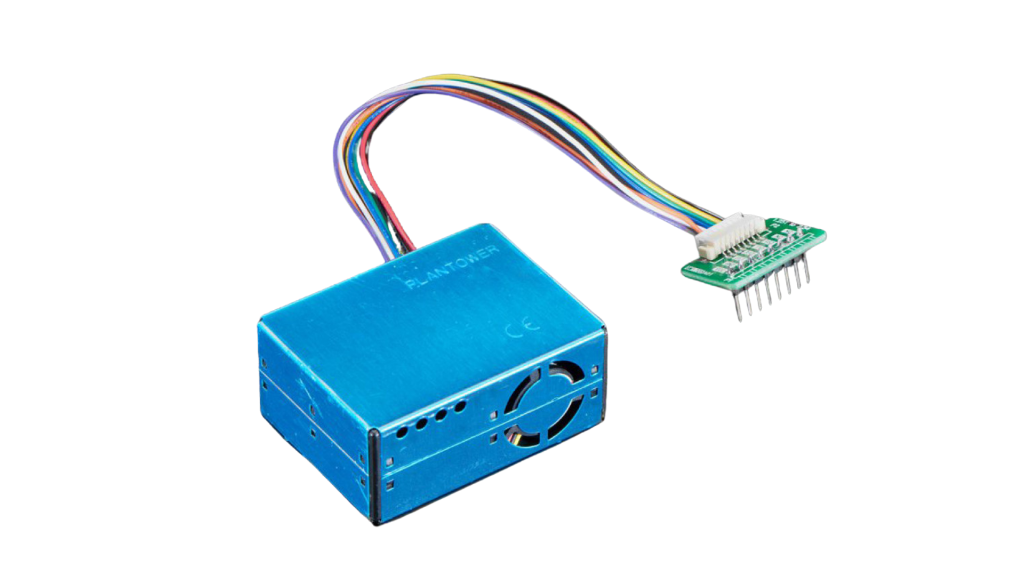
\includegraphics[width=0.95\linewidth]{images/pms5003.png}}\vspace*{2mm} & \vspace*{2mm}\makebox[\linewidth][c]{\includegraphics[width=0.95\linewidth]{images/gp2y1010au0f.png}}\vspace*{2mm} \\
        \hline
        \textbf{Nguyên lý đo} & Tán xạ LASER chủ động + quạt hút & Tán xạ LASER chủ động + quạt hút & LED hồng ngoại, không có quạt hút \\
        \hline
        \textbf{Dải đo} & PM2.5, PM10 (0--1000\,$\mu$g/m$^3$) & PM1.0, PM2.5, PM10 (0--500\,$\mu$g/m$^3$) & Chỉ có độ nhạy 0.5V/0.1mg/m$^3$ \\
        \hline
        \textbf{Đầu ra tín hiệu} & UART 9600bps / PWM & UART 9600bps & Analog (điện áp) \\
        \hline
        \textbf{Độ chính xác} & Sai số $\pm$10\% & Sai số $\pm$10$\mu$g/m$^3$ hoặc $\pm$10\% & Thấp, chỉ đo tương đối \\
        \hline
        \textbf{Nguồn điện} & 5V, $\sim$70mA (sleep $<$4mA) & 5V, $\leq$100mA (sleep $\leq$200$\mu$A) & 5V, $\sim$11mA \\
        \hline
        \textbf{Kích thước} & 71 $\times$ 70 $\times$ 23 mm (Lớn) & 50 $\times$ 38 $\times$ 21 mm (Trung bình) & 46 $\times$ 30 $\times$ 17.6 mm (Nhỏ gọn) \\
        \hline
        \textbf{Tuổi thọ} & $\sim$8000 giờ & $\geq$3 năm (MTTF) & Dài (không có quạt hút) \\
        \hline
        \textbf{Độ ẩm HĐ} & 0--70\% RH & 0--99\% RH & Không công bố \\
        \hline
    \end{tabular}
\caption{Bảng phân công công việc thực hiện dự án}
    \label{tab:work_distribution}
    \begin{tabularx}{\textwidth}{|l|>{\raggedright\arraybackslash}X|l|}
        \hline
        \textbf{Thành viên} & \textbf{Nhiệm vụ đảm nhiệm} & \textbf{Trạng thái} \\ 
        \hline
        Nguyễn Danh Trung & Thiết kế mạch nguyên lý PCB, hàn lắp linh kiện phần cứng, hiệu chuẩn các cảm biến BME680, PMS5003, MQ-135. & Hoàn thành \\ 
        \hline
        Tống Quang Giáp & Lập trình firmware trên ESP32, xây dựng thuật toán lọc số, tích hợp Watchdog Timer. & Hoàn thành \\ 
        \hline
        Nguyễn Huy Hoàng & Xây dựng giao diện hiển thị, giám sát dữ liệu thời gian thực, cấu hình REST API, triển khai cơ sở dữ liệu MongoDB Atlas và kết nối MQTT Broker. & Hoàn thành \\ 
        \hline
    \end{tabularx}
\end{table}

% ============================================================
%  CHƯƠNG 2. PHÂN TÍCH HỆ THỐNG
% ============================================================
\newpage
\begin{center}
    \textbf{\Large CHƯƠNG 2. PHÂN TÍCH HỆ THỐNG}
\end{center}
\addcontentsline{toc}{section}{CHƯƠNG 2. PHÂN TÍCH HỆ THỐNG}
\setcounter{section}{2}
\setcounter{subsection}{0}
\subsection{Yêu cầu chức năng}
Với vai trò là một hệ thống đo chất lượng không khí tự động, thiết bị cần đáp ứng các yêu cầu chức năng sau:

\subsubsection{Tự động thu thập dữ liệu cảm biến}
Hệ thống phải tự động đọc và thu thập các dữ liệu môi trường vật lý bao gồm nồng độ bụi mịn (PM2.5, PM10), nhiệt độ, độ ẩm, áp suất, chỉ số khí VOC, và nồng độ các loại khí độc hại khác từ các cụm cảm biến tương ứng.

\subsubsection{Cập nhật dữ liệu thời gian thực lên giao diện}
Thông tin đo được phải được hiển thị lên màn hình OLED cục bộ và truyền tải lên Web Dashboard trực tuyến với chu kỳ tự động cập nhật thời gian thực (dưới 10 giây/lần).

\subsubsection{Tính toán chính xác chỉ số chất lượng không khí}
Hệ thống phải tự động tính toán chỉ số chất lượng không khí AQI theo chuẩn US EPA từ các thông số bụi mịn và khí độc đo được, đưa ra các mức đánh giá trực quan.

\subsubsection{Cấp nguồn ổn định cho thiết bị}
Thiết bị sử dụng nguồn 5V DC qua jack nguồn tiện dụng, có cấu hình phân ly mạch nguồn tốt chống tự phát nhiệt gây sai số cho cảm biến nhiệt độ.

\subsubsection{Tối ưu hóa độ sai số và độ trễ}
Việc xử lý dữ liệu qua các bộ lọc số tại biên giúp hạn chế sai số, đồng thời thời gian truyền nhận từ cảm biến lên giao diện web phải đảm bảo độ trễ nhỏ hơn 10 giây.



\subsection{Yêu cầu phi chức năng}
Hệ thống cũng cần tuân thủ các chỉ tiêu phi chức năng để tăng tính thực tiễn:

\subsubsection{Giao diện sử dụng thân thiện}
Web Dashboard được thiết kế trực quan, dễ thao tác trên cả máy tính và thiết bị di động, tự động đổi màu sắc cảnh báo theo thang US EPA giúp người dùng dễ dàng nhận biết.

\subsubsection{Thiết kế nhỏ gọn}
Kích thước hộp chứa thiết bị và mạch PCB phải nhỏ gọn, thuận tiện cho việc lắp đặt ngoài trời hoặc trong nhà.

\subsubsection{Giá thành hợp lý}
Sử dụng các linh kiện phổ biến trên thị trường để tối ưu hóa chi phí sản xuất diện rộng.

\newpage
\begin{center}
    \textbf{\Large CHƯƠNG 3. THIẾT KẾ HỆ THỐNG}
\end{center}
\addcontentsline{toc}{section}{CHƯƠNG 3. THIẾT KẾ HỆ THỐNG}
\setcounter{section}{3}
\setcounter{subsection}{0}

\subsection{Tổng quan hệ thống}
Hệ thống được xây dựng dựa trên kiến trúc phân tầng 3 lớp IoT tiêu chuẩn: \textbf{Edge -- Fog -- Cloud}.

\begin{figure}[H]
    \centering
    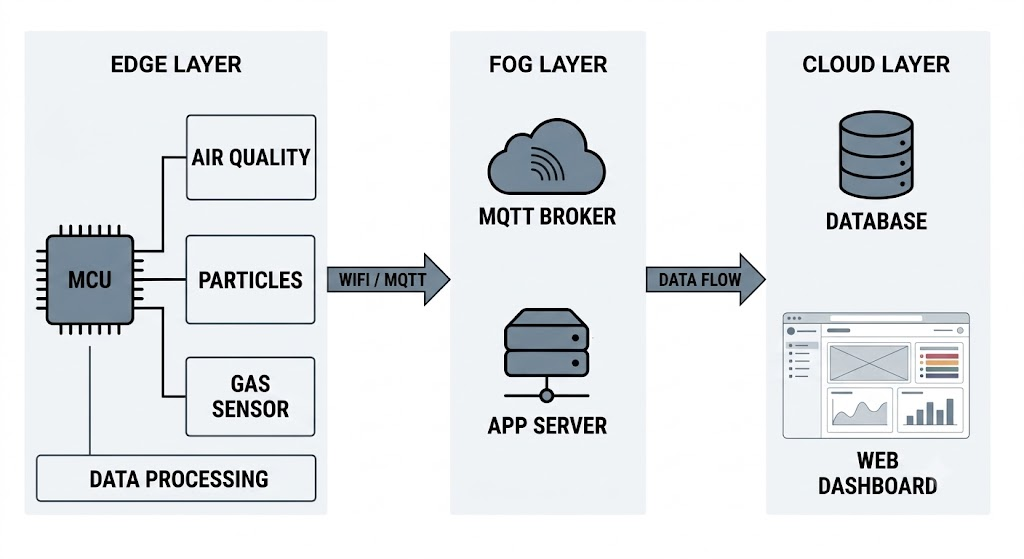
\includegraphics[width=0.9\textwidth]{images/block_diagram.png}
    \caption{Cấu trúc tổng quan của hệ thống trạm quan trắc IoT}
    \label{fig:system_overview}
\end{figure}

Hệ thống bao gồm các thành phần chính sau:
\begin{itemize}
    \item \textbf{Tầng biên (Edge)}: Vi điều khiển kết nối trực tiếp với các cảm biến để thu thập dữ liệu môi trường, thực hiện lọc nhiễu và tính toán chỉ số chất lượng không khí ngay tại thiết bị đầu cuối.
    \item \textbf{Tầng trung gian (Fog)}: Lớp trung chuyển đảm nhận việc định tuyến, chuẩn hóa dữ liệu và bổ sung nhãn thời gian thông qua giao thức truyền thông nhẹ và dịch vụ xử lý trung gian.
    \item \textbf{Tầng đám mây (Cloud)}: Cơ sở dữ liệu lưu trữ dữ liệu lịch sử lâu dài, kết hợp giao diện web hiển thị biểu đồ trực quan và cảnh báo cho người dùng.
\end{itemize}

\subsection{Nguyên lý hoạt động}

\begin{figure}[H]
    \centering
    % \includegraphics[width=0.9\textwidth]{images/system_flow.png}
    \textbf{[CHÈN SƠ ĐỒ NGUYÊN LÝ HOẠT ĐỘNG VÀO ĐÂY]}
    \caption{Sơ đồ nguyên lý hoạt động của hệ thống}
    \label{fig:system_flow}
\end{figure}

Hệ thống hoạt động theo chu trình liên tục, khép kín qua 4 bước chính:
\begin{enumerate}
    \item \textbf{Thu thập \& Xử lý tại biên (Edge Processing):} Mỗi 10 giây, ESP32 thực hiện đọc song song dữ liệu thô từ ba cảm biến. Dữ liệu được lọc số qua bộ lọc Trung vị, Trung bình động và EMA để khử nhiễu và làm mượt trước khi đưa vào tính toán.
    \item \textbf{Truyền tải IoT (MQTT Publish):} ESP32 đóng gói dữ liệu đã xử lý thành gói tin JSON, bổ sung siêu dữ liệu (metadata) và publish lên topic \texttt{aqistation/data} trên broker MQTT qua kết nối WiFi.
    \item \textbf{Lưu trữ đám mây (Cloud Storage):} Dịch vụ backend Node.js (chạy liên tục trên Vercel) subscribe topic \texttt{aqistation/data}, nhận gói tin, bổ sung nhãn thời gian phía server (Server-side Timestamping) và ghi bản ghi vào MongoDB Atlas.
    \item \textbf{Hiển thị \& Cảnh báo (Web Dashboard):} Ứng dụng Next.js tự động làm mới giao diện mỗi 5 giây bằng cách gọi REST API nội bộ để lấy dữ liệu mới nhất từ MongoDB và cập nhật biểu đồ, chỉ số AQI, trạng thái cảnh báo lên màn hình người dùng.
\end{enumerate}

\subsection{So sánh và lựa chọn linh kiện}
Để tối ưu hóa chi phí và đảm bảo độ chính xác kỹ thuật, nhóm đã thực hiện so sánh chi tiết giữa các giải pháp linh kiện trên thị trường:


\subsubsection{Cảm biến bụi mịn}
Cảm biến bụi mịn là thành phần quan trọng nhất của trạm đo chất lượng không khí:

Qua bảng so sánh, nhóm quyết định lựa chọn \textbf{PMS5003} vì độ chính xác vượt trội, khả năng phân tách chi tiết các dải kích thước bụi và tín hiệu đầu ra số tin cậy, hoàn toàn xứng đáng với giá thành đầu tư cho một trạm quan trắc.

\subsubsection{Cảm biến đo khí độc}
Để đo đạc các loại khí độc hại trong không khí, nhóm đã tiến hành so sánh các dòng cảm biến phổ biến thuộc họ MQ:

\begin{table}[H]
    \centering
    \begin{tabular}{|>{\raggedright\arraybackslash}p{3.5cm}|>{\raggedright\arraybackslash}p{3.5cm}|>{\raggedright\arraybackslash}p{3.5cm}|>{\raggedright\arraybackslash}p{4cm}|}
        \hline
        \textbf{Tiêu chí} & \textbf{MQ-135} & \textbf{MQ-7} & \textbf{MQ-4} \\
        \hline
        & \vspace*{2mm}\makebox[\linewidth][c]{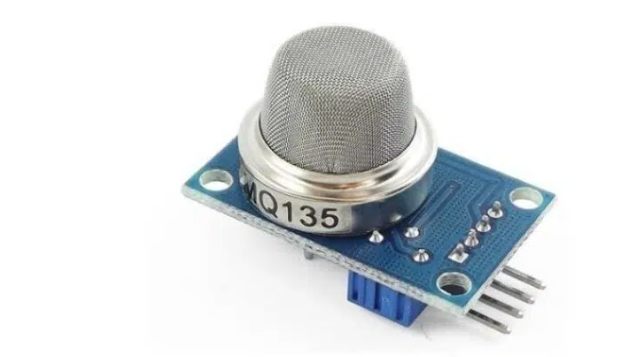
\includegraphics[width=0.95\linewidth]{images/mq135.png}}\vspace*{2mm} & \vspace*{2mm}\makebox[\linewidth][c]{\includegraphics[width=0.95\linewidth]{images/mq7.png}}\vspace*{2mm} & \vspace*{2mm}\makebox[\linewidth][c]{\includegraphics[width=0.95\linewidth]{images/mq4.png}}\vspace*{2mm} \\
        \hline
        \textbf{Khí mục tiêu chính} & NH$_3$, benzen, cồn, khói & Carbon monoxide (CO) & Methane (CH$_4$) / khí thiên nhiên \\
        \hline
        \textbf{Dải đo} & 10--1000\,ppm & 20--2000\,ppm & 200--10.000\,ppm \\
        \hline
        \textbf{Độ chọn lọc} & Thấp (phổ rộng, nhiều khí) & Trung bình (chọn lọc CO tốt) & Trung bình (chọn lọc methane) \\
        \hline
        \textbf{Chế độ đốt nóng} & 5V liên tục & Luân phiên 5V/1.4V (2 pha) & 5V liên tục \\
        \hline
        \textbf{Thời gian làm nóng} & 2--3 phút & 2.5 phút (1 chu kỳ đo) & 2--3 phút \\
        \hline
        \textbf{Công suất tiêu thụ} & $\sim$900\,mW & $\sim$350\,mW (trung bình) & $\sim$900\,mW \\
        \hline
        \textbf{Phát hiện CO} & Kém & Xuất sắc & Kém \\
        \hline
        \textbf{Phát hiện Methane} & Kém & Kém & Xuất sắc \\
        \hline
    \end{tabular}
\caption{So sánh các dòng cảm biến đo khí độc}
    \label{tab:ss_mq}
    \vspace{0.2cm}
    
\end{table}

Qua bảng so sánh, nhóm quyết định lựa chọn \textbf{MQ-135} do khả năng phát hiện phổ rộng các loại khí độc hại phổ biến trong không khí, cấu hình phần cứng đơn giản (chỉ cần cấp nguồn 5V liên tục thay vì luân phiên như MQ-7) và đáp ứng tốt nhu cầu quan trắc môi trường tổng hợp.

\subsubsection{Cảm biến vi khí hậu}
Để đo đạc các thông số vi khí hậu (nhiệt độ, độ ẩm, áp suất) và bù trừ sai số cho cảm biến khí, nhóm đã tiến hành so sánh các dòng cảm biến của hãng Bosch:

\begin{table}[H]
    \centering
    \begin{tabular}{|>{\raggedright\arraybackslash}p{3cm}|>{\raggedright\arraybackslash}p{3.5cm}|>{\raggedright\arraybackslash}p{4cm}|>{\raggedright\arraybackslash}p{4.5cm}|}
        \hline
        \textbf{Tiêu chí} & \textbf{BMP280} & \textbf{BME280} & \textbf{BME680} \\
        \hline
        & \vspace*{2mm}\makebox[\linewidth][c]{\includegraphics[width=0.95\linewidth]{images/bmp280.png}}\vspace*{2mm} & \vspace*{2mm}\makebox[\linewidth][c]{\includegraphics[width=0.95\linewidth]{images/bme280.png}}\vspace*{2mm} & \vspace*{2mm}\makebox[\linewidth][c]{\includegraphics[width=0.95\linewidth]{images/bme680.png}}\vspace*{2mm} \\
        \hline
        \textbf{Thông số đo} & Nhiệt độ, áp suất (không có độ ẩm, VOC) & Nhiệt độ, áp suất, độ ẩm & Nhiệt độ, áp suất, độ ẩm, khí VOC (4-in-1) \\
        \hline
        \textbf{Độ chính xác} & Áp suất $\pm 1$\,hPa, nhiệt độ $\pm 1.0^\circ$C & Độ ẩm $\pm 3\%$, áp suất $\pm 1$\,hPa, nhiệt độ $\pm 1.0^\circ$C & Độ ẩm $\pm 3\%$, áp suất $\pm 1$\,hPa, nhiệt độ $\pm 1.0^\circ$C (tương đương BME280) \\
        \hline
        \textbf{Điện áp / giao tiếp} & 1.71--3.6V, I2C hoặc SPI & 1.71--3.6V, I2C hoặc SPI & 1.71--3.6V (VDD), 1.2--3.6V (VDDIO), I2C hoặc SPI \\
        \hline
        \textbf{Kích thước / công suất} & Nhỏ gọn, tiêu thụ điện rất thấp & Nhỏ gọn, công suất thấp, tương tự BMP280 & Gói LGA $3.0 \times 3.0$\,mm, dòng đo gas 0.09--12\,mA tùy chế độ, sleep mode $0.15\,\mu$A \\
        \hline
        \textbf{Giá thành} & Rẻ nhất trong 3 loại & Nhỉnh hơn BMP280 & Đắt nhất, do tích hợp thêm cảm biến khí MOX \\
        \hline
    \end{tabular}
\caption{So sánh các dòng cảm biến vi khí hậu}
    \label{tab:ss_bme}
    \vspace{0.2cm}
    
\end{table}

Qua phân tích, nhóm quyết định lựa chọn \textbf{BME680} vì sự vượt trội với khả năng đo thêm khí VOC trên một module cực kỳ nhỏ gọn, đáp ứng hoàn hảo yêu cầu đo đạc chất lượng không khí tổng hợp.

\subsubsection{Module truyền thông và vi điều khiển}
\begin{itemize}
    \item \textbf{Arduino Uno R3}: Chỉ có vi điều khiển 8-bit, bộ nhớ SRAM rất nhỏ (2\,KB), không tích hợp WiFi, không thể chạy đa nhiệm FreeRTOS ổn định.
    \item \textbf{STM32F103C8T6}: Vi điều khiển 32-bit Cortex-M3 mạnh mẽ, bộ nhớ lớn nhưng không tích hợp sẵn kết nối mạng không dây WiFi, cần thêm module ESP8266 ngoài làm phức tạp mạch.
    \item \textbf{ESP32-WROOM-32D}: Tích hợp sẵn bộ thu phát WiFi 2.4\,GHz và Bluetooth, CPU Dual-core Xtensa 32-bit mạnh mẽ hoạt động ở 240\,MHz, hỗ trợ hoàn hảo hệ điều hành thời gian thực FreeRTOS, dung lượng SRAM 520\,KB dồi dào. Nhóm quyết định lựa chọn \textbf{ESP32}.
\end{itemize}

\subsection{Danh sách linh kiện cần sử dụng}
Dưới đây là chi tiết thông số kỹ thuật của các linh kiện đã lựa chọn:

\subsubsection{Giới thiệu về mô đun ESP32 DOIT DevKit V1}
Vi điều khiển trung tâm ESP32 (phiên bản mô đun DOIT DevKit V1) đóng vai trò bộ não điều khiển toàn bộ hệ thống trạm đo chất lượng không khí, chịu trách nhiệm đọc dữ liệu từ các cảm biến, lọc và xử lý tín hiệu, tính toán chỉ số AQI và truyền dữ liệu lên cloud qua giao thức MQTT.

\begin{table}[H]
    \centering
    \begin{tabular}{|>{\raggedright\arraybackslash}p{4.0cm}|>{\raggedright\arraybackslash}p{7.5cm}|}
\hline
 & \centering\arraybackslash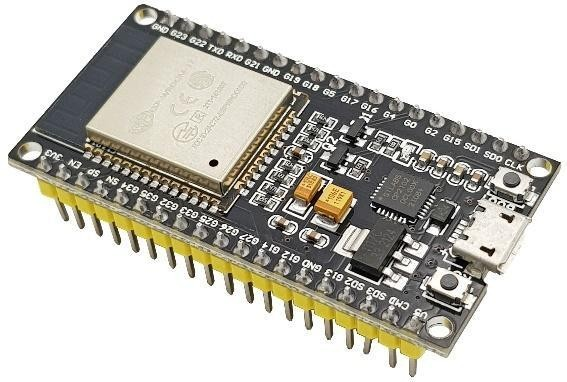
\includegraphics[width=0.28]{images/esp32.png} \\ 
        \hline
MCU & Xtensa@ Dual-Core 32-bit LX6 600 DMIPS \\ 
        \hline
Điện áp nguồn & 5V DC \\ 
        \hline
Đầu vào/ra điện áp & 3.3V DC \\ 
        \hline
Băng tần & 80 - 240 MHz \\ 
        \hline
Giao thức WiFi & 802.11B/g/n/E/I (802.11N @ 2.4 GHz lên đến 150 Mbit/s) \\ 
        \hline
Tần số WiFi & 2.4 -- 2.5 GHz \\ 
        \hline
Bluetooth & V4.2 - BLE \\ 
        \hline
Bộ nhớ & 448 Kbyte ROM, 520 Kbyte SRAM, 6 Kbyte SRAM trên RTC và QSPI Hỗ trợ đèn flash / SRAM chip \\ 
        \hline
Chip USB-Serial & CP2102 \\ 
        \hline
Anten không dây & PCB \\ 
        \hline
Giá thành & 200.000VNĐ \\ 
        \hline\end{tabular}
\caption{Thông số ESP32 DOIT DevKit V1}
    \label{tab:ss_pm}
    \vspace{0.2cm}
    
\end{table}

\subsubsection{Giới thiệu về cảm biến bụi PMS5003}
\noindent\textbf{Tìm hiểu về các phép đo PM:}\\[6pt]
Một hạt bụi (Particulate Matter -- PM) là hỗn hợp của chất rắn và giọt chất lỏng, kích thước hiển vi, có thể trôi nổi trong không khí. Chúng có thể có nhiều hình dạng, kích cỡ và cấu tạo từ nhiều chất khác nhau. 
\begin{itemize}
    \item \textbf{PM1.0}: Những hạt có đường kính nhỏ hơn 1 micromet.
    \item \textbf{PM2.5}: Những hạt có đường kính từ 1 đến 2.5 micromet.
    \item \textbf{PM10}: Những hạt có đường kính từ 2.5 đến 10 micromet.
\end{itemize}

\noindent\textbf{Nguyên lý hoạt động}\\[6pt]
Cảm biến PMS5003 hoạt động dựa trên nguyên lý tán xạ ánh sáng laser chủ động. Khi các hạt bụi lơ lửng trong không khí được hút vào buồng đo thông qua quạt tích hợp, chúng đi qua chùm tia laser. Ánh sáng tán xạ từ hạt bụi được cảm biến quang học thu nhận và chuyển đổi thành tín hiệu điện. Vi điều khiển tích hợp trên cảm biến sử dụng thuật toán dựa trên lý thuyết Mie để tính toán đường kính tương đương của các hạt bụi và số lượng hạt trên một đơn vị thể tích, từ đó đưa ra nồng độ khối lượng PM1.0, PM2.5, PM10 chuẩn xác.

\vspace{12pt}
\noindent\begin{minipage}{\textwidth}
\noindent\textbf{Thông số kỹ thuật}\\[6pt]
 
\begin{table}[H]
 \centering
 \begin{tabular}{|>{\raggedright\arraybackslash}p{4.0cm}|>{\raggedright\arraybackslash}p{7.5cm}|}
 \hline
 \textbf{Thông số} & \textbf{Giá trị} \\ 
        \hline
 Điện áp hoạt động & 4.95\,V -- 5.05\,V DC \\ 
        \hline
 Dòng điện tối đa & 120\,mA \\ 
        \hline
 Dòng điện chờ & $\leq 200\,\mu$A \\ 
        \hline
 Giao tiếp & UART (9600 baud, 8N1) \\ 
        \hline
 Dải đo PM & 0 -- 500\,$\mu$g/m$^3$ \\ 
        \hline
 Độ phân giải PM & 1\,$\mu$g/m$^3$ \\ 
        \hline
 Kích thước hạt nhỏ nhất & 0.3\,$\mu$m \\ 
        \hline
 Thời gian đáp ứng & $<$ 10 giây \\ 
        \hline
 Nhiệt độ hoạt động & -10\,$^\circ$C đến +60\,$^\circ$C \\ 
        \hline
 Độ ẩm hoạt động & 0 -- 99\% RH \\ 
        \hline
 Kích thước & 50 $\times$ 38 $\times$ 21\,mm \\ 
        \hline
 Tuổi thọ & $\geq$ 3 năm \\ 
        \hline
 \end{tabular}
\caption{Thông số kỹ thuật cảm biến PMS5003}
 \label{tab:pms5003_specs}
 
 \end{table}
\end{minipage}
\vspace{12pt}

\noindent\textbf{Sơ đồ chân của module}\\[6pt]
 \begin{figure}[H]
     \centering
     \includegraphics[width=0.45\textwidth]{images/pms5003_pinout.png}
     \caption{Sơ đồ chân giao tiếp của PMS5003}
     \label{fig:pms5003_pinout}
 \end{figure}
 
 \begin{table}[H]
 \centering
 \begin{tabular}{|c|c|l|}
 \hline
 \textbf{Chân} & \textbf{Ký hiệu} & \textbf{Mô tả chức năng} \\ 
        \hline
 1 & VCC & Nguồn dương (5V) \\ 
        \hline
 2 & GND & Nguồn âm (Mass) \\ 
        \hline
 3 & SET & Pin thiết lập chế độ chờ. Mức cao: hoạt động. Mức thấp: chờ. \\ 
        \hline
 4 & RX & Nhận dữ liệu (để nhận lệnh điều khiển nếu có) \\ 
        \hline
 5 & TX & Truyền dữ liệu (cung cấp dữ liệu đo PM ra ngoài) \\ 
        \hline
 6 & RESET & Pin khởi động lại module. Mức thấp: reset. \\ 
        \hline
 7,8 & NC & Không kết nối \\ 
        \hline
 \end{tabular}
\caption{Chức năng các chân của PMS5003}
 \label{tab:pms5003_pins}
 
 \end{table}

\noindent\textbf{Thuật toán đọc cảm biến PMS5003}\\[6pt]
Về mặt phần cứng, giao tiếp UART của lõi ESP32 tự động sao chép các byte nhận được vào một vùng đệm. Ở phần mềm ứng dụng, vi điều khiển sẽ định kỳ kiểm tra vùng đệm này để lấy dữ liệu. Vì cảm biến PMS5003 gửi dữ liệu liên tục thành từng gói 32-byte mà không có ký tự ngắt rõ ràng, phần mềm cần một thuật toán để dò tìm đúng 2 byte bắt đầu (0x42 và 0x4D), sau đó mới đọc tiếp đủ 30 byte còn lại. Thuật toán thu thập và giải mã dữ liệu này được mô tả trực quan qua lưu đồ dưới đây:

\begin{figure}[H]
\centering
\begin{tikzpicture}[node distance=0.6cm and 1.2cm,
  block/.style={rectangle, draw, rounded corners=4pt, fill=blue!10, text width=3cm, align=center, minimum height=0.9cm, font=\small},
  decision/.style={diamond, draw, fill=orange!15, text width=2.2cm, align=center, aspect=1.6, font=\small},
  arrow/.style={->, >=stealth, thick}]
  \node[block] (wait) {Chờ dữ liệu\\(Tìm byte\\bắt đầu)};
  \node[decision, below=0.7cm of wait] (chk42) {Byte nhận\\= 0x42?};
  \node[decision, right=1.8cm of chk42] (chk4D) {Byte tiếp theo\\= 0x4D?};
  \node[block, below=0.7cm of chk4D] (read32) {Thu thập đủ\\32 byte khung};
  \node[decision, below=0.7cm of read32] (chksum) {Checksum\\hợp lệ?};
  \node[block, right=1.8cm of chksum] (discard) {Loại bỏ gói lỗi\\quay lại từ đầu};
  \node[block, below=0.7cm of chksum] (decode) {Giải mã trường\\PM1.0,\\PM2.5, PM10};
  \draw[arrow] (wait) -- (chk42);
  \draw[arrow] (chk42) -- node[above, font=\scriptsize]{Có} (chk4D);
  \draw[arrow] (chk42.west) -- +(-0.7,0) |- node[left, font=\scriptsize, pos=0.25]{Không} (wait.west);
  \draw[arrow] (chk4D) -- node[right, font=\scriptsize]{Có} (read32);
  \draw[arrow] (chk4D.north) -- +(0,0.5) -| node[above right, font=\scriptsize, pos=0.1]{Không} (wait.north);
  \draw[arrow] (read32) -- (chksum);
  \draw[arrow] (chksum) -- node[above, font=\scriptsize]{Không} (discard);
  \draw[arrow] (discard.north) |- (wait.east);
  \draw[arrow] (chksum) -- node[right, font=\scriptsize]{Có} (decode);
\end{tikzpicture}
\caption{Lưu đồ thuật toán đọc dữ liệu PMS5003}
\label{fig:pms_fsm}
\end{figure}

Cơ chế kiểm tra lỗi (Checksum) đóng vai trò rất quan trọng để phát hiện và loại bỏ các gói dữ liệu bị sai lệch do nhiễu đường truyền. Cách tính là lấy tổng của 30 byte đầu tiên để so sánh với 2 byte Checksum ở cuối gói. Sau khi gói dữ liệu được xác nhận là hợp lệ, nồng độ bụi mịn sẽ được trích xuất tại các vị trí tương ứng: PM2.5 nằm ở byte số 10--11 và PM10 nằm ở byte số 12--13. Ngoài ra, để chương trình không bị treo khi cảm biến đột ngột mất kết nối, thuật toán có cài đặt thời gian chờ tối đa (timeout). Nếu chờ quá lâu mà chưa nhận đủ 32 byte, hệ thống sẽ tự động hủy bỏ gói dữ liệu dang dở này và quay lại bước ban đầu để dò tìm gói mới.


\subsubsection{Giới thiệu về cảm biến khí BME680}

\noindent\textbf{Nguyên lý hoạt động}\\[6pt]
BME680 sử dụng công nghệ MEMS (Hệ thống vi cơ điện tử) cho phép tích hợp 4 cảm biến vào cùng một package nhỏ. Nhiệt độ và độ ẩm đóng vai trò tham chiếu quan trọng để bù sai số (nhiệt-ẩm bù trừ) cho các cảm biến hóa học nhạy khí vốn dễ bị trôi giá trị đo khi môi trường thay đổi.

\vspace{12pt}
\noindent\begin{minipage}{\textwidth}
\noindent\textbf{Thông số kỹ thuật}\\[6pt]

\begin{table}[H]
\centering
\begin{tabular}{|>{\raggedright\arraybackslash}p{4.0cm}|>{\raggedright\arraybackslash}p{7.5cm}|}
\hline
\textbf{Thông số} & \textbf{Giá trị} \\
\hline
Điện áp hoạt động & 1.71 -- 3.6\,V \\
\hline
Giao tiếp & I2C và SPI \\
\hline
Dải đo nhiệt độ & -40 -- +85$^\circ$C \\
\hline
Dải đo độ ẩm & 0 -- 100\% \\
\hline
Dải đo áp suất & 300 -- 1100\,hPa \\
\hline
Đo VOC (Khí hữu cơ) & BIAQ index \\
\hline
Kích thước & $3.0 \times 3.0 \times 0.93$\,mm \\
\hline
\end{tabular}
\caption{Thông số kỹ thuật cảm biến BME680}
\label{tab:bme680_specs}

\end{table}
\end{minipage}
\vspace{12pt}

\noindent\textbf{Sơ đồ chân của module}\\[6pt]
 \begin{figure}[H]
     \centering
     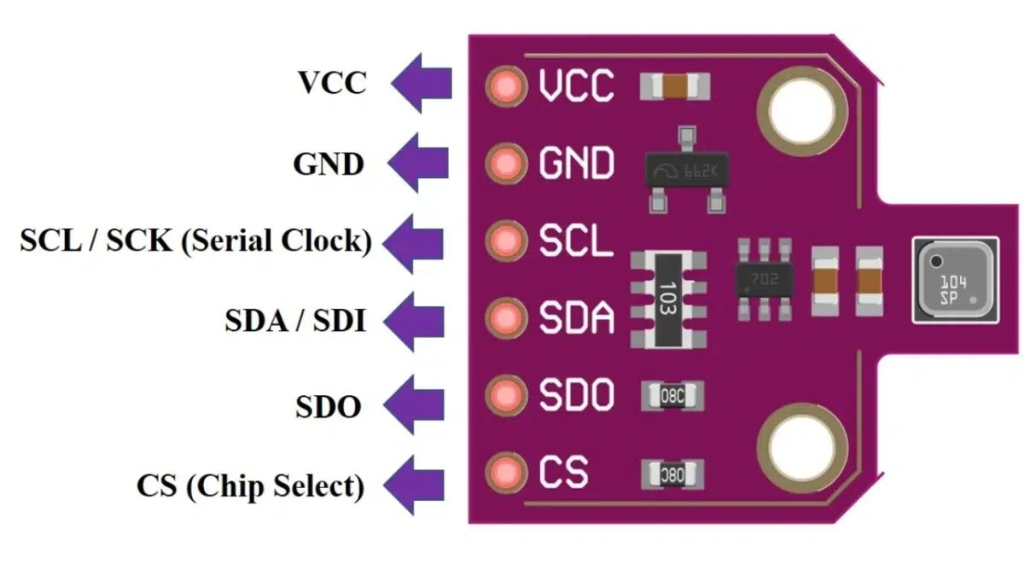
\includegraphics[width=0.45\textwidth]{images/bme680_pinout.png}
     \caption{Sơ đồ chân module cảm biến BME680}
     \label{fig:bme680_pinout}
 \end{figure}

\noindent\textbf{Thuật toán đọc cảm biến BME680}\\[6pt]
Vi điều khiển ESP32 đóng vai trò là I2C Master, định kỳ giao tiếp với BME680 ở địa chỉ `0x76` hoặc `0x77`. Phần mềm sẽ gửi tín hiệu Start kèm thanh ghi cần đọc. Cảm biến sau đó tính toán nhiệt độ, độ ẩm, áp suất và khí VOC rồi lưu vào thanh ghi. Sau khi vi điều khiển đọc dữ liệu, các thuật toán nội suy và lọc số (như lọc trung bình trượt lũy thừa - EMA) được áp dụng ở tầng ứng dụng để giảm thiểu độ trôi của giá trị đo trước khi đóng gói gửi đi.


\subsubsection{Giới thiệu về cảm biến MQ-135}

\noindent\textbf{Nguyên lý hoạt động}\\[6pt]
Cảm biến MQ-135 thuộc họ cảm biến khí bán dẫn (Semiconductor Gas Sensor) sử dụng vật liệu SnO$_2$ (Thiếc đioxit) làm màng nhạy khí. Khi hoạt động trong không khí sạch, màng SnO$_2$ có độ dẫn điện thấp. Khi tồn tại các khí ô nhiễm hoặc khí độc hại như Amoniac (NH$_3$), Benzen, Cồn, Khói, hay Carbon Dioxide (CO$_2$) trong môi trường, độ dẫn điện của cảm biến sẽ tăng lên tỷ lệ thuận với nồng độ khí.

\vspace{12pt}
\noindent\begin{minipage}{\textwidth}
\noindent\textbf{Thông số kỹ thuật}\\[6pt]

\begin{table}[H]
\centering
\begin{tabular}{|l|c|l|}
\hline
\textbf{Thông số} & \textbf{Ký hiệu} & \textbf{Giá trị} \\
\hline
Loại cảm biến & --- & Bán dẫn (SnO$_2$) \\
\hline
Khí mục tiêu & --- & Amoniac, sunfua, benzen, khói \\
\hline
Phạm vi phát hiện & --- & 10 $\sim$ 1000\,ppm \\
\hline
Điện áp nguồn/sấy & Vc / VH & 5.0\,V $\pm$ 0.1\,V (AC/DC) \\
\hline
Công suất tiêu thụ & PH & $\leq$ 950\,mW \\
\hline
Điện trở sấy & RH & 30\,$\Omega$ $\pm$ 3\,$\Omega$ (ở nhiệt độ phòng) \\
\hline
Thời gian làm nóng & --- & Trên 48 giờ \\
\hline
\end{tabular}
\caption{Thông số kỹ thuật cảm biến MQ-135}
\label{tab:mq135_specs_new}

\end{table}
\end{minipage}
\vspace{12pt}

\noindent\textbf{Sơ đồ chân của module}\\[6pt]
 \begin{figure}[H]
     \centering
     \includegraphics[width=0.55\textwidth]{images/mq135_module.png}
     \caption{Module cảm biến khí MQ-135 và kích thước cơ học}
     \label{fig:mq135_module}
 \end{figure}

\noindent\textbf{Thuật toán đọc cảm biến MQ-135}\\[6pt]
Khí cảm nhận được MQ-135 chuyển đổi thành mức điện áp đầu ra analog trên chân AO. Chân này được kết nối với một kênh ADC (Analog-to-Digital Converter) của vi điều khiển ESP32 (ở độ phân giải 12-bit). Để hạn chế nhiễu điện áp và dao động đọc lường, hệ thống sẽ đọc đa mẫu (multi-sampling) và áp dụng bộ lọc trung vị (Median Filter) để loại trừ các giá trị dị thường trước khi đưa ra kết quả điện áp đại diện cuối cùng.

\subsection{Thiết kế phần cứng}

\subsubsection{Thiết kế mạch nguyên lý}
Để thiết kế phần cứng cho trạm đo, nhóm phát triển phân tách sơ đồ đấu nối chân thành các mạch chức năng riêng biệt:

\paragraph{Mạch cảm biến bụi PMS5003}\mbox{}\\
Cảm biến PMS5003 giao tiếp qua UART2 của ESP32. Chân TX (chân 2) của PMS5003 được kết nối với GPIO16 (RX2) của ESP32; chân RX (chân 1) nối với GPIO17 (TX2). Nguồn nuôi 5V được cấp trực tiếp từ chân VIN của ESP32 để chạy quạt hút bụi của cảm biến.

Sơ đồ kết nối chi tiết giữa ESP32 và cảm biến PMS5003 được thể hiện trong Bảng~\ref{tab:schematic_pms5003}:

\begin{table}[H]
    \centering
    \begin{tabular}{|c|c|}
        \hline
        \textbf{Chân ESP32} & \textbf{Chân PMS5003} \\
        \hline
        GPIO16 (RX2) & Pin 5 (TX) \\
        \hline
        GPIO17 (TX2) & Pin 4 (RX) \\
        \hline
        VIN (5V) & Pin 1 (VCC) \\
        \hline
        GND & Pin 2 (GND) \\
        \hline
    \end{tabular}
    \caption{Bảng kết nối PMS5003 và ESP32}
    \label{tab:schematic_pms5003}
\end{table}

\paragraph{Mạch cảm biến vi khí hậu BME680}\mbox{}\\
BME680 sử dụng giao tiếp I2C. Chân SDA được nối với GPIO21, chân SCL nối với GPIO22 của ESP32. Nguồn cấp cho chip BME680 lấy trực tiếp từ đường 3.3V (chân 3V3) của ESP32 để bảo vệ mạch MEMS. Khi khởi động, firmware tự động quét lần lượt hai địa chỉ I2C khả dĩ của module (\texttt{0x76} và \texttt{0x77}) để tự nhận diện đúng địa chỉ mà không cần cấu hình cứng, tăng tính linh hoạt khi thay thế module cảm biến.

Sơ đồ kết nối chi tiết giữa ESP32 và cảm biến BME680 được thể hiện trong Bảng~\ref{tab:schematic_bme680}:

\begin{table}[H]
    \centering
    \begin{tabular}{|c|c|}
        \hline
        \textbf{Chân ESP32} & \textbf{Chân BME680} \\
        \hline
        GPIO21 (SDA) & Pin 4 (SDA) \\
        \hline
        GPIO22 (SCL) & Pin 3 (SCL) \\
        \hline
        3.3V (3V3) & Pin 1 (VCC) \\
        \hline
        GND & Pin 2 (GND) \\
        \hline
    \end{tabular}
    \caption{Bảng kết nối BME680 và ESP32}
    \label{tab:schematic_bme680}
\end{table}

\subparagraph{Hiệu chỉnh sai số tự phát nhiệt}\mbox{}\\
Trong quá trình đo đạc khí VOC, BME680 kích hoạt bộ sấy nội bộ ở nhiệt độ khoảng $320^\circ$C để oxy hóa các phân tử khí hữu cơ bay hơi. Nhiệt lượng tỏa ra từ bộ sấy này, kết hợp với nhiệt lượng tỏa ra từ chính vi xử lý ESP32 đặt gần cảm biến trên cùng bo mạch PCB, khiến giá trị nhiệt độ môi trường đọc được từ BME680 luôn cao hơn thực tế khoảng $2$--$4^\circ$C. Qua khảo sát và đối chiếu hơn 31.000 bản ghi dữ liệu thực nghiệm liên tục, nhóm ghi nhận nhiệt độ trung bình đo được là $32.96^\circ$C trong khi điều kiện phòng thực tế tại Việt Nam trong giai đoạn đo dao động khoảng $29$--$31^\circ$C. Do đó, firmware áp dụng một hệ số bù trừ cố định $-3.0^\circ$C được cộng trực tiếp vào giá trị nhiệt độ thô trước khi đưa qua bộ lọc EMA, giúp đưa giá trị hiển thị về sát với điều kiện môi trường thực tế hơn. Hệ số bù này được xác định bằng thực nghiệm so sánh với nhiệt kế tham chiếu và có thể tinh chỉnh lại nếu triển khai trạm đo tại vị trí hoặc điều kiện tản nhiệt PCB khác.

\paragraph{Mạch cảm biến khí độc MQ-135}\mbox{}\\
Chân AOUT của MQ-135 được nối tới chân ADC1\_CH6 (GPIO34) của ESP32 qua một cầu phân áp để hạ điện áp tín hiệu tối đa từ 5V xuống 3.3V, đảm bảo dải đo tuyến tính an toàn của bộ chuyển đổi ADC trên ESP32.

Sơ đồ kết nối chi tiết giữa ESP32 và cảm biến MQ-135 thông qua cầu phân áp được thể hiện trong Bảng~\ref{tab:schematic_mq135}:

\begin{table}[H]
    \centering
    \begin{tabular}{|c|c|}
        \hline
        \textbf{Chân ESP32} & \textbf{Chân MQ-135} \\
        \hline
        GPIO34 (ADC1) & AO (qua cầu phân áp) \\
        \hline
        VIN (5V) & VCC (5V) \\
        \hline
        GND & GND \\
        \hline
    \end{tabular}
    \caption{Bảng kết nối MQ-135 và ESP32}
    \label{tab:schematic_mq135}
\end{table}

\paragraph{Toàn mạch}\mbox{}\\
Toàn bộ sơ đồ mạch nguyên lý của hệ thống được minh họa dưới đây:

\begin{figure}[H]
    \centering
    \includegraphics[width=1.0\textwidth]{images/schematic_diagram.png}
    \caption{Sơ đồ mạch nguyên lý toàn hệ thống}
    \label{fig:schematic_diagram}
\end{figure}

\subsubsection{Phân tích công suất}
Việc tính toán và phân tích công suất tiêu thụ của hệ thống giúp thiết kế nguồn cấp DC phù hợp và ổn định cho trạm quan trắc hoạt động lâu dài:

\paragraph{Cảm biến bụi mịn PMS5003}\mbox{}\\
Cảm biến PMS5003 tiêu thụ dòng điện trung bình khoảng $100\,\text{mA}$ ở mức điện áp nguồn $5\,\text{V}$ khi quạt hút hoạt động liên tục. Công suất tiêu thụ tương ứng là:
\[
P_{\text{PMS}} = 5\,\text{V} \times 0.1\,\text{A} = 0.5\,\text{W}
\]

\paragraph{Cảm biến vi khí hậu BME680}\mbox{}\\
Cảm biến BME680 cực kỳ tiết kiệm năng lượng. Ở chế độ đo tối đa, dòng điện tiêu thụ chỉ khoảng $15\,\mu\text{A}$ ở điện áp $3.3\,\text{V}$. Tuy nhiên khi bộ sấy gia nhiệt khí VOC hoạt động, dòng điện tăng lên tối đa $12\,\text{mA}$. Công suất tiêu thụ lúc gia nhiệt cực đại là:
\[
P_{\text{BME}} = 3.3\,\text{V} \times 0.012\,\text{A} \approx 0.04\,\text{W}
\]

\paragraph{Cảm biến khí độc MQ-135}\mbox{}\\
Cảm biến MQ-135 sử dụng một dây sấy gia nhiệt nội bộ để duy trì nhiệt độ màng ô-xít kim loại. Dòng điện sấy yêu cầu liên tục khoảng $150\,\text{mA}$ ở điện áp $5\,\text{V}$. Công suất tiêu thụ tương đối lớn:
\[
P_{\text{MQ135}} = 5\,\text{V} \times 0.15\,\text{A} = 0.75\,\text{W}
\]

\paragraph{Vi xử lý ESP32}\mbox{}\\
ESP32 tiêu thụ dòng điện biến thiên mạnh tùy thuộc vào trạng thái truyền sóng RF. Khi WiFi hoạt động và truyền gói tin MQTT, dòng điện tiêu thụ đỉnh có thể đạt $240\,\text{mA}$ ở điện áp $3.3\,\text{V}$. Công suất tiêu thụ đỉnh là:
\[
P_{\text{ESP32}} = 3.3\,\text{V} \times 0.24\,\text{A} \approx 0.8\,\text{W}
\]

\paragraph{Tính toán công suất tổng}\mbox{}\\
Tổng công suất tiêu thụ cực đại của toàn hệ thống là:
\[
P_{\text{Tổng}} = P_{\text{PMS}} + P_{\text{BME}} + P_{\text{MQ135}} + P_{\text{ESP32}} \approx 0.5 + 0.04 + 0.75 + 0.8 \approx 2.09\,\text{W}
\]
Với công suất tổng khoảng $2.1\,\text{W}$, hệ thống yêu cầu một adapter nguồn điện cấp tối thiểu $5\,\text{V} - 1\,\text{A}$ (tương đương $5\,\text{W}$) để đảm bảo hệ thống hoạt động ổn định và an toàn, tránh sụt áp đột ngột khi truyền WiFi.

\subsubsection{Kết nối vi xử lý ESP32 với các module}
Toàn bộ các cảm biến của trạm quan trắc được kết nối trực tiếp với vi điều khiển trung tâm ESP32 thông qua ba chuẩn giao tiếp khác nhau (UART, I2C, ADC tương tự). Phần dưới đây trình bày chi tiết bảng kết nối chân của từng module.

\subsection{Công nghệ và phần mềm nhúng}

\subsubsection{Hệ điều hành FreeRTOS}
Hệ thống sử dụng cơ chế đa nhiệm thời gian thực FreeRTOS:
Để đảm bảo hệ thống thu thập dữ liệu đa cảm biến hoạt động với độ trễ thấp, ổn định và không xảy ra hiện tượng mất mát dữ liệu truyền thông, thiết kế hệ thống tận dụng tối đa kiến trúc phần cứng của vi xử lý trung tâm ESP32 và hệ điều hành thời gian thực FreeRTOS.

\paragraph{Kiến trúc phần cứng vi xử lý ESP32}\mbox{}\\

Trạm gateway được xây dựng trên mô đun ESP32 DOIT DevKit V1. Đây là bộ não trung tâm của toàn bộ trạm quan trắc, do đó nhóm tiến hành phân tích sâu về vi kiến trúc của chip nhằm khai thác tối đa hiệu năng phần cứng và đưa ra các quyết định thiết kế phần mềm phù hợp.

\begin{itemize}
    \item \textbf{Cấu trúc Dual-Core Harvard}: Bộ xử lý trung tâm gồm hai nhân xử lý độc lập Xtensa Dual-Core 32-bit LX6 hoạt động với tần số xung nhịp lên tới 240\,MHz, mỗi nhân hoạt động độc lập theo kiến trúc Harvard (tách biệt bus lệnh và bus dữ liệu), cho phép nạp lệnh và truy xuất dữ liệu diễn ra đồng thời trong cùng một chu kỳ xung nhịp. Mỗi nhân LX6 có pipeline 5 tầng và tập lệnh mật độ cao Xtensa ISA hỗ trợ cả lệnh 16-bit và 24-bit nhằm tối ưu hóa dung lượng mã chương trình.
    \item \textbf{Đơn vị dấu phẩy động (FPU)}: Mỗi nhân tích hợp sẵn khối tính toán số thực dấu phẩy động đơn, giúp tăng tốc đáng kể các phép tính nội suy tuyến tính trong thuật toán AQI và các bộ lọc số mà không cần mô phỏng số thực bằng phần mềm.
    \item \textbf{Bộ chuyển đổi tương tự - số (ADC)}: ESP32 trang bị hai bộ ADC xấp xỉ liên tiếp 12-bit là ADC1 và ADC2 với tổng cộng 18 kênh đo. Trong hệ thống, kênh ADC1\_CH6 (GPIO34) được sử dụng để đọc điện áp tương tự từ cảm biến MQ-135.
\end{itemize}

\paragraph{Bản đồ bộ nhớ và tổ chức không gian địa chỉ}\mbox{}\\

Việc hiểu rõ tổ chức bộ nhớ của ESP32 là yếu tố quyết định để thiết kế phần mềm nhúng hiệu quả, tránh hiện tượng tràn ngăn xếp khi chạy đồng thời nhiều Task FreeRTOS. ESP32 tổ chức không gian địa chỉ theo mô hình phân vùng như sau:

\begin{table}[H]
\centering\small
\caption{Bản đồ bộ nhớ của vi xử lý ESP32}
\label{tab:esp32_memmap}

\end{table}

Trong thiết kế firmware của trạm quan trắc, cấu trúc dữ liệu chia sẻ \texttt{SharedData} (chứa các trường PM2.5, PM10, nhiệt độ, độ ẩm, áp suất, giá trị MQ-135 và AQI tổng hợp) được cấp phát tĩnh trong vùng DRAM, có kích thước cố định nhỏ hơn 200\,byte, đảm bảo không chiếm dụng quá nhiều tài nguyên SRAM vốn cũng phải phục vụ cho ngăn xếp giao thức mạng TCP/IP (LwIP) và bộ đệm mã hóa TLS khi cần mở rộng bảo mật kết nối MQTT trong tương lai.

\paragraph{Hệ thống ngắt và ma trận định tuyến ngắt}\mbox{}\\

ESP32 sở hữu một bộ điều phối ngắt linh hoạt gọi là Ma trận Ngắt, cho phép ánh xạ tùy ý 71 nguồn tín hiệu ngắt phần cứng khác nhau (ngoại vi UART, I2C, GPIO, Timer, RF...) tới 32 đường ngắt CPU nội bộ của mỗi nhân xử lý, với 7 mức độ ưu tiên khác nhau. Đặc tính này đóng vai trò quan trọng trong việc đảm bảo độ trễ đáp ứng thấp cho tác vụ đọc dữ liệu UART từ cảm biến PMS5003:

\begin{itemize}
    \item Khi bộ đệm phần cứng FIFO của UART2 nhận đủ số byte ngưỡng cấu hình (Receive FIFO Threshold), một tín hiệu ngắt phần cứng \texttt{UART\_INTR} được kích hoạt và định tuyến qua Ma trận Ngắt tới nhân CPU 1 (Core 1) -- nơi đang chạy \texttt{taskPMS}.
    \item Ngắt UART được cấu hình ở mức ưu tiên cao (Priority Level 3), đảm bảo hàm xử lý ngắt (ISR) được nhân xử lý phục vụ gần như ngay lập tức, hạn chế tình trạng tràn bộ đệm phần cứng có thể làm mất byte dữ liệu và phá vỡ tính toàn vẹn của khung truyền 32-byte từ PMS5003.
    \item Ngắt Watchdog Timer và ngắt Timer hệ thống (Tick Timer phục vụ bộ lập lịch FreeRTOS, chu kỳ 1\,ms) được cấu hình ở mức ưu tiên cao nhất (Priority Level 7 - Non-Maskable), đảm bảo cơ chế giám sát lỗi hoạt động ngay cả khi các tác vụ khác đang chiếm dụng CPU.
\end{itemize}

\paragraph{Cây xung nhịp và cơ chế định thời}\mbox{}\\

Hệ thống xung nhịp của ESP32 được tổ chức phân cấp bắt đầu từ thạch anh ngoài tần số 40\,MHz. Tín hiệu này được đưa qua bộ nhân tần số PLL nội bộ để tạo ra các mức xung nhịp phục vụ những khối chức năng khác nhau:

\begin{table}[H]
\centering\small
\caption{Cấu hình cây xung nhịp phục vụ các khối chức năng của ESP32}
\label{tab:clock_tree}
\begin{tabular}{|>{\raggedright\arraybackslash}p{4.0cm}|>{\raggedright\arraybackslash}p{2.5cm}|>{\raggedright\arraybackslash}p{6.5cm}|}
\hline
\textbf{Khối chức năng} & \textbf{Tần số} & \textbf{Vai trò trong hệ thống} \\ 
        \hline
CPU Clock (hai nhân LX6) & 240\,MHz & Xung nhịp chính cho xử lý tính toán: lọc số, tính AQI, đóng gói JSON. \\ 
        \hline
APB Bus Clock & 80\,MHz & Xung nhịp cấp cho các ngoại vi kết nối qua bus APB: UART, I2C, GPIO, Timer. \\ 
        \hline
RTC Clock (Nội bộ 150\,kHz hoặc XTAL 32.768\,kHz) & 32.768\,kHz & Duy trì đồng hồ thời gian thực trong các chế độ ngủ (đề xuất dùng cho hướng phát triển Deep Sleep). \\ 
        \hline\end{tabular}
\end{table}

Việc APB Bus Clock hoạt động ổn định ở 80\,MHz đảm bảo tốc độ Baudrate của UART2 (9600\,bps giao tiếp với PMS5003) và tốc độ xung Clock của I2C (400\,kHz Fast-mode giao tiếp với BME680) được tạo ra với sai số cực nhỏ (dưới 0.5\%), tránh hiện tượng trôi tốc độ truyền có thể gây lỗi khung truyền khi hoạt động liên tục trong thời gian dài.

\paragraph{Đặc tính và hiệu chuẩn bộ chuyển đổi ADC}\mbox{}\\

Bộ ADC nội bộ của ESP32, đặc biệt là kênh ADC1 sử dụng để đọc cảm biến MQ-135, có một số đặc tính phi tuyến cần được phân tích và hiệu chỉnh để đảm bảo độ chính xác phép đo:

\begin{itemize}
    \item \textbf{Độ suy hao đầu vào}: ADC1 hỗ trợ 4 mức suy hao cấu hình được (0\,dB, 2.5\,dB, 6\,dB, 11\,dB), quyết định dải điện áp đo tuyến tính. Với tín hiệu MQ-135 sau cầu phân áp có biên độ tối đa gần 3.3\,V, nhóm cấu hình mức suy hao 11\,dB để mở rộng dải đo tuyến tính lên đến khoảng 0 -- 3.3\,V.
    \item \textbf{Sai số phi tuyến tại vùng biên}: Đặc tính chuyển đổi thực tế của ADC ESP32 không hoàn toàn tuyến tính ở hai đầu dải đo (gần 0\,V và gần điện áp tối đa), sai lệch có thể lên tới 5--7\% so với giá trị lý thuyết nếu không hiệu chỉnh.
    \item \textbf{Hiệu chuẩn bằng eFuse Vref}: ESP32 lưu trữ sẵn trong vùng nhớ eFuse (bộ nhớ ghi một lần cấp bởi nhà sản xuất) giá trị điện áp tham chiếu nội bộ (Vref) đã được đo đạc và hiệu chỉnh riêng cho từng chip tại nhà máy. Firmware truy xuất giá trị Vref này để tính toán bảng tra cứu chuyển đổi ADC-điện áp chính xác hơn, giảm sai số hệ thống xuống dưới 2\%.
\end{itemize}

\paragraph{Quản lý năng lượng và các chế độ hoạt động}\mbox{}\\

ESP32 hỗ trợ nhiều chế độ hoạt động với mức tiêu thụ năng lượng khác nhau, cho phép cân bằng giữa hiệu năng xử lý và tuổi thọ nguồn cấp:

\begin{table}[H]
\centering\small
\caption{Các chế độ quản lý năng lượng của ESP32}
\label{tab:power_modes}
\begin{tabular}{|>{\raggedright\arraybackslash}p{3.0cm}|>{\raggedright\arraybackslash}p{3.0cm}|>{\raggedright\arraybackslash}p{6.2cm}|}
\hline
\textbf{Chế độ} & \textbf{Dòng tiêu thụ điển hình} & \textbf{Trạng thái hoạt động của CPU và ngoại vi} \\ 
        \hline
Active Mode & 80 -- 260\,mA & Cả hai nhân CPU hoạt động đầy đủ, module WiFi/RF thu phát liên tục. Đây là chế độ trạm quan trắc sử dụng xuyên suốt để đảm bảo độ trễ truyền dữ liệu dưới 10 giây. \\ 
        \hline
Modem-sleep & 3 -- 20\,mA & CPU vẫn hoạt động ở tần số đầy đủ nhưng module RF tạm ngắt giữa các chu kỳ Beacon, chỉ bật lại theo lịch trình Access Point. \\ 
        \hline
Light-sleep & 0.8\,mA & CPU tạm dừng xung nhịp, ngoại vi và RF tắt, bộ nhớ RAM vẫn được giữ nguyên trạng thái. Đánh thức bằng ngắt ngoài hoặc Timer. \\ 
        \hline
Deep-sleep & 10\,$\mu$A & Chỉ còn lõi RTC hoạt động để duy trì đồng hồ và bộ nhớ RTC Memory, toàn bộ CPU chính và RAM SRAM bị ngắt điện hoàn toàn. Đây là chế độ được đề xuất áp dụng cho hướng phát triển tích hợp năng lượng mặt trời trong tương lai. \\ 
        \hline\end{tabular}
\end{table}

Hiện tại, trạm quan trắc được thiết kế để hoạt động liên tục ở chế độ Active Mode nhằm đảm bảo tính tức thời của dữ liệu giám sát; việc khai thác các chế độ tiết kiệm năng lượng sâu hơn được nhóm đề xuất là hướng phát triển trong tương lai khi tích hợp nguồn năng lượng mặt trời độc lập.

\paragraph{Cơ chế truy cập bộ nhớ trực tiếp DMA cho ngoại vi}\mbox{}\\

Để giảm tải cho CPU trong quá trình truyền nhận dữ liệu khối lượng lớn qua các bus ngoại vi, ESP32 tích hợp bộ điều khiển truy cập bộ nhớ trực tiếp dùng chung cho các ngoại vi tốc độ cao. Đối với giao tiếp I2C với cảm biến BME680, thư viện driver có thể tùy chọn sử dụng kênh DMA để tự động sao chép dữ liệu từ thanh ghi ngoại vi vào vùng nhớ DRAM mà không cần CPU can thiệp từng byte, giúp giải phóng chu kỳ xử lý cho các tác vụ tính toán AQI và lọc số khác đang chạy song song trên cùng nhân CPU.

\paragraph{Cấu hình đa nhiệm FreeRTOS và cơ chế lập lịch}\mbox{}\\

Hệ điều hành thời gian thực FreeRTOS được tích hợp sẵn trong nhân mở rộng Arduino ESP32 Core, cho phép lập trình đa nhiệm trực quan trên nền tảng Arduino IDE. Cơ chế lập lịch của FreeRTOS hoạt động theo thuật toán lập lịch ưu tiên trưng dụng, kết hợp chia sẻ thời gian cho các tác vụ có cùng mức ưu tiên.

Để khai thác tối đa cấu trúc Dual-Core, hệ thống sử dụng hàm khởi tạo tác vụ ghim nhân \texttt{xTaskCreatePinnedToCore()} để phân bổ các Task FreeRTOS lên các nhân CPU phù hợp (như đã tóm tắt ở Bảng~\ref{tab:freertos_gw}):
\begin{enumerate}
    \item \textbf{Nhân CPU 1 (Core 1) - Chuyên trách phần cứng đầu cuối}:
    \begin{itemize}
        \item \texttt{taskPMS} (Mức ưu tiên 3 - Cao nhất): Do cảm biến PMS5003 gửi luồng dữ liệu liên tục 32-byte ở tốc độ 9600\,baud qua UART, việc bỏ lỡ một byte sẽ làm sai lệch kiểm tra Checksum và mất đồng bộ khung truyền. Do đó, tác vụ này được đặt ở mức ưu tiên cao nhất trên Core 1 để giải phóng bộ đệm nhận UART kịp thời.
        \item \texttt{taskSensors} (Mức ưu tiên 2): Đảm nhiệm việc đọc dữ liệu chu kỳ từ BME680 (I2C) và MQ-135 (ADC). Việc đọc các cảm biến này diễn ra định kỳ 10 giây/lần nên tác vụ này có thể ở mức ưu tiên thấp hơn \texttt{taskPMS}.
    \end{itemize}
    \item \textbf{Nhân CPU 0 (Core 0) - Chuyên trách mạng và truyền thông}:
    \begin{itemize}
        \item \texttt{taskNetwork} (Mức ưu tiên 1): Nhân Core 0 là nơi hệ thống chạy các tiến trình nền của chip WiFi và ngăn xếp giao thức TCP/IP. Việc ghim tác vụ truyền thông MQTT lên Core 0 giúp tránh các ngắt truyền thông không dây làm ảnh hưởng đến tính chính xác về thời gian của các thuật toán xử lý dữ liệu ngoại vi chạy trên Core 1.
    \end{itemize}
\end{enumerate}

\begin{table}[H]
\centering\small
\caption{Bảng phân bổ Task FreeRTOS lên hai nhân xử lý của ESP32}
\label{tab:freertos_gw}
\begin{tabular}{|l|c|c|>{\raggedright\arraybackslash}p{5.2cm}|}
\hline
\textbf{Task} & \textbf{Nhân (Core)} & \textbf{Ưu tiên} & \textbf{Chu kỳ / Điều kiện thực thi} \\ 
        \hline
\texttt{taskPMS} & Core 1 & 3 (Cao nhất) & Ngắt-hướng theo FIFO UART2, xử lý ngay khi có dữ liệu \\ 
        \hline
\texttt{taskSensors} & Core 1 & 2 & Định kỳ 10\,giây/lần (I2C + ADC polling) \\ 
        \hline
\texttt{taskNetwork} & Core 0 & 1 & Sự kiện-hướng, đánh thức bởi \texttt{dataReadyEvent} \\ 
        \hline
Idle Task (hệ thống) & Core 0 \& Core 1 & 0 (Thấp nhất) & Chạy khi không có Task nào sẵn sàng, phục vụ dọn rác bộ nhớ FreeRTOS \\ 
        \hline\end{tabular}
\end{table}

Sơ đồ dưới đây minh họa trực quan việc phân bổ tác vụ lên hai nhân xử lý và luồng đồng bộ hóa dữ liệu giữa chúng thông qua vùng nhớ dùng chung \texttt{SharedData}:

\begin{figure}[H]
\centering
\begin{tikzpicture}[node distance=0.55cm and 1.5cm,
  block/.style={rectangle, draw, rounded corners=3pt, fill=gray!15, text width=2.8cm, align=center, minimum height=0.85cm, font=\small},
  coreblock/.style={rectangle, draw, rounded corners=3pt, fill=blue!20, text width=2.8cm, align=center, minimum height=0.85cm, font=\small\bfseries},
  shared/.style={rectangle, draw, rounded corners=3pt, fill=green!15, text width=2.8cm, align=center, minimum height=0.85cm, font=\small},
  arrow/.style={->, >=stealth, thick},
  dasharrow/.style={->, >=stealth, thick, dashed}]
  % Core 1
  \node[coreblock] (core1) {CORE 1\\Xử lý cảm biến};
  \node[block, below=0.6cm of core1] (taskPMS) {taskPMS\\Ưu tiên 3\\(ngắt UART2)};
  \node[block, below=0.6cm of taskPMS] (taskSensors) {taskSensors\\Ưu tiên 2\\(I2C + ADC, 10s)};
  % Core 0
  \node[coreblock, right=3.0cm of core1] (core0) {CORE 0\\Xử lý mạng};
  \node[block, below=0.6cm of core0] (taskNetwork) {taskNetwork\\Ưu tiên 1};
  % Shared
  \node[shared, below=0.6cm of taskSensors, xshift=2.2cm] (shared) {SharedData\\(bảo vệ bởi\\Mutex)};
  % Arrows
  \draw[arrow] (core1) -- (taskPMS);
  \draw[arrow] (taskPMS) -- (taskSensors);
  \draw[arrow] (core0) -- (taskNetwork);
  \draw[arrow] (taskPMS.east) -- ++(0.4,0) |- (taskNetwork.west);
  \draw[arrow] (taskSensors.east) -- ++(0.4,0) -- (shared.west);
  \draw[dasharrow] (shared.east) -- ++(0.4,0) |- node[right, font=\scriptsize]{Event Group\\BIT\_MQTT\_READY} (taskNetwork.south);
\end{tikzpicture}
\caption{Lưu đồ phân bổ tác vụ Dual-Core}
\label{fig:dualcore_flow}
\end{figure}

\paragraph{Cơ chế đồng bộ hóa luồng dữ liệu và loại trừ tranh chấp}\mbox{}\\

Do các tác vụ hoạt động song song trên hai nhân xử lý độc lập và truy cập chung vào cấu trúc dữ liệu \texttt{systemData}, nguy cơ xảy ra tranh chấp dữ liệu là rất cao. Để bảo vệ tính toàn vẹn của dữ liệu, hệ thống áp dụng các cơ chế đồng bộ hóa:
\begin{itemize}
    \item \textbf{Cơ chế khóa Mutex}: Sử dụng một biến loại trừ tương hỗ \texttt{dataMutex} kiểu \texttt{SemaphoreHandle\_t}. Trước khi thực hiện thao tác ghi dữ liệu (ở \texttt{taskPMS}, \texttt{taskSensors}) hoặc thao tác đọc dữ liệu để đóng gói JSON (ở \texttt{taskNetwork}), tác vụ đó bắt buộc phải chiếm quyền giữ khóa thông qua hàm \texttt{xSemaphoreTake()}. Sau khi hoàn tất thao tác, khóa được giải phóng bằng hàm \texttt{xSemaphoreGive()}. Điều này ngăn ngừa hiện tượng xung đột khi một tác vụ đang đọc dữ liệu chưa hoàn chỉnh trong khi tác vụ khác đang cập nhật đè lên.
    \item \textbf{Cơ chế thông báo hướng sự kiện bằng Event Groups}: Để tránh việc tác vụ truyền thông \texttt{taskNetwork} liên tục kiểm tra vòng lặp gây lãng phí năng lượng và tài nguyên CPU, hệ thống sử dụng một nhóm sự kiện \texttt{dataReadyEvent}. Khi \texttt{taskSensors} tính toán xong chỉ số AQI tổng hợp, nó sẽ đánh dấu sự kiện bằng cách set bit \texttt{BIT\_MQTT\_READY} qua hàm \texttt{xEventGroupSetBits()}. Tác vụ \texttt{taskNetwork} lúc này đang ở trạng thái chờ bị chặn bởi hàm \texttt{xEventGroupWaitBits()} sẽ lập tức được đánh thức để thực thi đóng gói và gửi dữ liệu lên MQTT Broker, tối ưu hóa hiệu suất làm việc của vi điều khiển.
\end{itemize}

\paragraph{Cơ chế giám sát chịu lỗi Watchdog Timer}\mbox{}\\

Nhằm bảo đảm tính tin cậy tuyệt đối khi thiết bị hoạt động lâu dài tại hiện trường mà không cần can thiệp vật lý, hệ thống tích hợp bộ giám sát lỗi phần cứng Watchdog Timer cấp vi điều khiển:
\begin{itemize}
    \item Hệ thống cấu hình Task Watchdog Timer (TWDT) giám sát các luồng hoạt động chính của FreeRTOS trên cả hai nhân xử lý.
    \item Định kỳ trong vòng lặp vô hạn của mỗi Task, hàm xóa chó canh phòng \texttt{esp\_task\_wdt\_reset()} phải được gọi để báo hiệu tác vụ vẫn đang hoạt động bình thường.
    \item Nếu xảy ra hiện tượng treo tác vụ (do mất kết nối mạng bị block không thoát được hoặc lỗi deadlock tranh chấp tài nguyên), vi điều khiển sẽ không thể reset watchdog kịp thời. Khi hết thời gian cấu hình \texttt{WDT\_TIMEOUT\_S} (30 giây), phần cứng Watchdog sẽ kích hoạt ngắt Reset hệ thống, đưa ESP32 khởi động lại sạch sẽ để tự phục hồi hoạt động.
\end{itemize}

Lưu đồ dưới đây minh họa cơ chế giám sát Watchdog Timer song song với cơ chế tự động kết nối lại mạng WiFi/MQTT, được thực thi độc lập trên nhân Core 0 mà không làm gián đoạn các Task đọc cảm biến trên Core 1:

\begin{figure}[H]
\centering
\begin{tikzpicture}[node distance=0.6cm and 1.5cm,
  block/.style={rectangle, draw, rounded corners=4pt, fill=gray!15, text width=3cm, align=center, minimum height=0.9cm, font=\small},
  decision/.style={diamond, draw, fill=orange!15, text width=2.4cm, align=center, aspect=1.6, font=\small},
  alarm/.style={rectangle, draw, rounded corners=4pt, fill=red!20, text width=3cm, align=center, minimum height=0.9cm, font=\small},
  action/.style={rectangle, draw, rounded corners=4pt, fill=purple!15, text width=3cm, align=center, minimum height=0.9cm, font=\small},
  arrow/.style={->, >=stealth, thick}]
  \node[block] (loop) {Vòng lặp\\giám sát\\(mỗi Task)};
  \node[decision, below=0.8cm of loop] (ok) {Task hoàn\\thành chu kỳ\\đúng hạn?};
  \node[action, below=0.7cm of ok] (reset) {Gọi\\\texttt{esp\_task\_wdt\_reset()}\\(nạp lại bộ\\đếm WDT)};
  \node[block, right=2.0cm of ok] (hang) {Task bị treo};
  \node[decision, below=0.8cm of hang] (timeout) {Quá 30 giây\\không nạp\\lại WDT?};
  \node[alarm, below=0.7cm of timeout] (reboot) {Kích hoạt\\Hardware Reset\\Khởi động\\lại ESP32};
  \draw[arrow] (loop) -- (ok);
  \draw[arrow] (ok) -- node[right, font=\scriptsize]{Có} (reset);
  \draw[arrow] (reset.north) -- ++(0,0.3) -| (loop.south);
  \draw[arrow] (ok) -- node[above, font=\scriptsize]{Không} (hang);
  \draw[arrow] (hang) -- (timeout);
  \draw[arrow] (timeout) -- node[right, font=\scriptsize]{Có} (reboot);
  \draw[arrow] (timeout.east) -- ++(0.7,0) |- node[right, font=\scriptsize, pos=0.25]{Chưa} (hang.east);
\end{tikzpicture}
\caption{Lưu đồ hoạt động Watchdog Timer}
\label{fig:wdt_flowchart}
\end{figure}

\subsubsection{Arduino IDE}
Lập trình Firmware được triển khai trên nền tảng phần mềm Arduino IDE thông qua lõi mở rộng ESP32 Core. Các thư viện nguồn mở chính thức được tích hợp bao gồm:
\begin{itemize}
    \item \texttt{Adafruit\_BME680}: Đọc và hiệu chuẩn thông số khí hậu và điện trở khí VOC từ cảm biến BME680 qua giao tiếp I2C.
    \item \texttt{PubSubClient}: Kết nối client nhẹ, bảo đảm truyền tải gói tin MQTT QoS 1 đến Broker.
    \item \texttt{ArduinoJson}: Thư viện tối ưu hóa bộ nhớ chuyên dụng dùng để serialize dữ liệu thành chuỗi JSON siêu nhẹ trước khi publish.
    \item \texttt{WiFi}, \texttt{WebServer}, \texttt{DNSServer}, \texttt{Preferences}: Bộ thư viện lõi ESP32 phục vụ module quản lý kết nối WiFi tự cấu hình, được trình bày chi tiết ở mục tiếp theo.
\end{itemize}

\subsubsection{Quản lý kết nối WiFi và trang cấu hình}

Một hạn chế phổ biến của các thiết bị IoT giá rẻ là việc cấu hình thông tin WiFi (SSID, mật khẩu) phải được ghi cứng trực tiếp vào mã nguồn firmware trước khi nạp, gây bất tiện lớn khi triển khai thiết bị tại nhiều địa điểm khác nhau có hạ tầng mạng khác nhau. Để giải quyết vấn đề này, nhóm phát triển đã tận dụng các ngoại vi có sẵn trên chip ESP32 (bộ nhớ Flash phân vùng NVS, lõi vô tuyến WiFi hỗ trợ đồng thời chế độ Access Point và Station) để xây dựng một module quản lý kết nối tự động, hoạt động độc lập với các Task xử lý cảm biến.

\paragraph{Cơ chế lưu trữ cấu hình bền vững trên phân vùng NVS}\mbox{}\\
ESP32 dành riêng một phân vùng bộ nhớ Flash gọi là NVS để lưu trữ dữ liệu dạng khóa-giá trị (key-value) tồn tại xuyên suốt các lần khởi động lại hoặc mất điện, khác biệt hoàn toàn với vùng nhớ RAM sẽ bị xóa trắng khi tắt nguồn. Thông qua thư viện \texttt{Preferences} (lớp trừu tượng hóa của NVS), thông tin SSID và mật khẩu WiFi mà người dùng nhập vào Cổng cấu hình được ghi trực tiếp xuống phân vùng Flash này, cho phép thiết bị tự động kết nối lại đúng mạng đã cấu hình ở những lần khởi động sau mà không cần lặp lại thao tác thiết lập.

\paragraph{Thứ tự ưu tiên kết nối ba tầng}\mbox{}\\
Để tối đa hóa khả năng tự phục hồi kết nối mà vẫn giữ được tính linh hoạt, firmware áp dụng chiến lược thử kết nối tuần tự theo ba tầng ưu tiên giảm dần, mỗi tầng có thời gian chờ tối đa (Timeout) riêng trước khi chuyển sang tầng kế tiếp:

\begin{enumerate}
    \item \textbf{Tầng 1 -- Thông tin lưu trong NVS}: Ưu tiên cao nhất, thử kết nối bằng thông tin đã lưu từ lần cấu hình gần nhất.
    \item \textbf{Tầng 2 -- Thông tin ghi cứng}: Nếu tầng 1 thất bại hoặc chưa từng cấu hình, thử kết nối bằng thông tin SSID/mật khẩu mặc định được nạp sẵn trong mã nguồn tại thời điểm biên dịch.
    \item \textbf{Tầng 3 -- Cổng cấu hình WiFi}: Nếu cả hai tầng trên đều thất bại, ESP32 tự chuyển chip WiFi sang chế độ kết hợp Access Point + Station (\texttt{WIFI\_AP\_STA}), tự phát ra một mạng WiFi riêng đặt tên theo địa chỉ MAC của thiết bị (đảm bảo tên mạng không trùng lặp giữa các trạm), đồng thời khởi chạy một máy chủ Web nội bộ (WebServer) và một máy chủ phân giải tên miền giả lập (DNS) chuyển hướng toàn bộ truy vấn tên miền về địa chỉ IP của chính ESP32. Cơ chế này lợi dụng tính năng phát hiện Captive Portal có sẵn trên hệ điều hành di động (thông qua các đường dẫn dò tìm đặc thù như \texttt{/generate\_204} của Android hay \texttt{/fwlink} của Windows) để tự động bật trình duyệt web hiển thị giao diện nhập mật khẩu WiFi ngay khi người dùng kết nối vào mạng do thiết bị phát ra, tương tự trải nghiệm đăng nhập WiFi công cộng tại quán cà phê hay sân bay.
\end{enumerate}

\begin{figure}[H]
\centering
\begin{tikzpicture}[node distance=0.55cm and 1.8cm,
  block/.style={rectangle, draw, rounded corners=4pt, fill=blue!10, text width=3.0cm, align=center, minimum height=0.85cm, font=\small},
  decision/.style={diamond, draw, fill=orange!15, text width=2.5cm, align=center, aspect=1.7, font=\small},
  success/.style={rectangle, draw, rounded corners=4pt, fill=green!20, text width=3.0cm, align=center, minimum height=0.85cm, font=\small},
  portal/.style={rectangle, draw, rounded corners=4pt, fill=gray!15, text width=3.0cm, align=center, minimum height=0.85cm, font=\small},
  arrow/.style={->, >=stealth, thick}]
  \node[block] (boot) {Khởi động};
  \node[decision, below=0.7cm of boot] (nvs) {Kết nối bằng\\thông tin NVS\\thành công?};
  \node[success, below=0.7cm of nvs] (ready) {Sẵn sàng\\hoạt động\\(chuyển sang\\WIFI\_STA)};
  \node[decision, right=2.2cm of nvs] (hard) {Kết nối bằng\\thông tin\\Hardcode\\thành công?};
  \node[portal, below=0.7cm of hard] (ap) {Bật Access Point\\+ WebServer\\+ DNS Server\\(Captive Portal)};
  \node[portal, below=0.7cm of ap] (wait) {Chờ người dùng\\chọn mạng và\\nhập mật khẩu\\qua trình duyệt};
  \node[portal, below=0.7cm of wait] (save) {Lưu SSID/Mật\\khẩu xuống\\phân vùng NVS};
  \draw[arrow] (boot) -- (nvs);
  \draw[arrow] (nvs) -- node[right, font=\scriptsize]{Có} (ready);
  \draw[arrow] (nvs) -- node[above, font=\scriptsize]{Không} (hard);
  \draw[arrow] (hard.south) -- node[right, font=\scriptsize]{Không} (ap);
  \draw[arrow] (hard.west) -- node[above, font=\scriptsize, pos=0.3]{Có} (ready.east);
  \draw[arrow] (ap) -- (wait);
  \draw[arrow] (wait) -- (save);
  \draw[arrow] (save.west) -- ++(-0.6,0) |- (ready.west);
\end{tikzpicture}
\caption{Lưu đồ kết nối WiFi 3 tầng}
\label{fig:wifi_flowchart}
\end{figure}

\paragraph{Phản hồi trạng thái bằng LED và nút cứng Reset cấu hình}\mbox{}\\
Để hỗ trợ người vận hành hiện trường không cần theo dõi log Serial, thiết bị tích hợp một đèn LED báo trạng thái (nhấp nháy chậm khi đang ở chế độ Cổng cấu hình, sáng ổn định khi đã kết nối thành công) điều khiển qua một chân GPIO rời. Đồng thời, nút bấm BOOT sẵn có trên board ESP32 được tái sử dụng làm nút reset cấu hình mềm: khi người dùng giữ nút này liên tục trong 5 giây, firmware sẽ xóa toàn bộ thông tin SSID/mật khẩu đã lưu trong NVS và khởi động lại thiết bị, đưa trạm quan trắc trở về trạng thái sẵn sàng cấu hình lại từ đầu -- hữu ích khi cần thay đổi mạng WiFi triển khai hoặc bàn giao thiết bị cho vị trí lắp đặt khác.

\subsection{Thiết kế phần mềm}

\subsubsection{Sơ đồ phân rã chức năng}
Cấu trúc chức năng của hệ thống phần mềm được mô hình hóa thông qua sơ đồ phân rã dưới đây:

\begin{figure}[H]
    \centering
    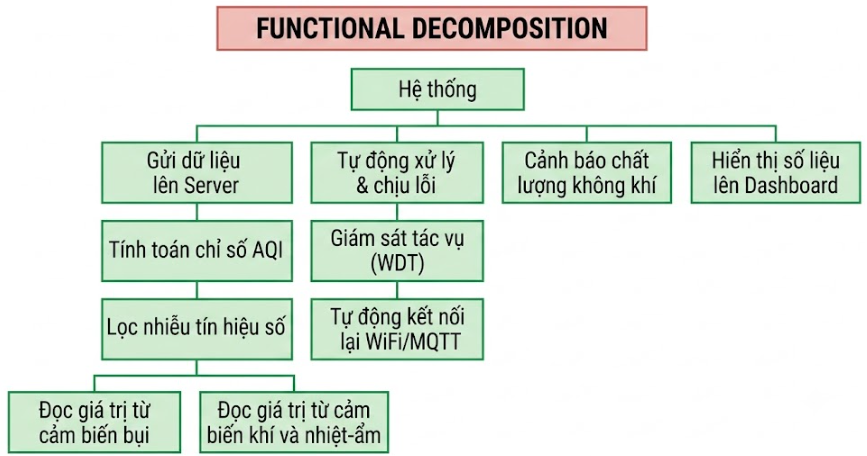
\includegraphics[width=0.85\textwidth]{images/functional_decomposition.png}
    \caption{Sơ đồ phân rã chức năng hệ thống}
    \label{fig:functional_decomposition}
\end{figure}

Sơ đồ trên phân định rõ các tác vụ xử lý thành 4 nhánh độc lập:
\begin{itemize}
    \item \textbf{Gửi dữ liệu lên Server}: Đọc cảm biến $\to$ lọc số $\to$ tính AQI $\to$ đóng gói gửi qua MQTT.
    \item \textbf{Tự động xử lý \& chịu lỗi}: Tự kết nối lại mạng và giám sát bằng Watchdog Timer.
    \item \textbf{Cảnh báo chất lượng không khí}: Xử lý ngưỡng theo chuẩn US EPA và cảnh báo tùy cấu hình.
    \item \textbf{Hiển thị số liệu Dashboard}: Giám sát trực quan dữ liệu thời gian thực và lịch sử.
\end{itemize}

\subsubsection{Biểu đồ tuần tự}
Luồng truyền nhận dữ liệu theo thời gian giữa các thành phần được thể hiện qua biểu đồ tuần tự:

\begin{figure}[H]
    \centering
    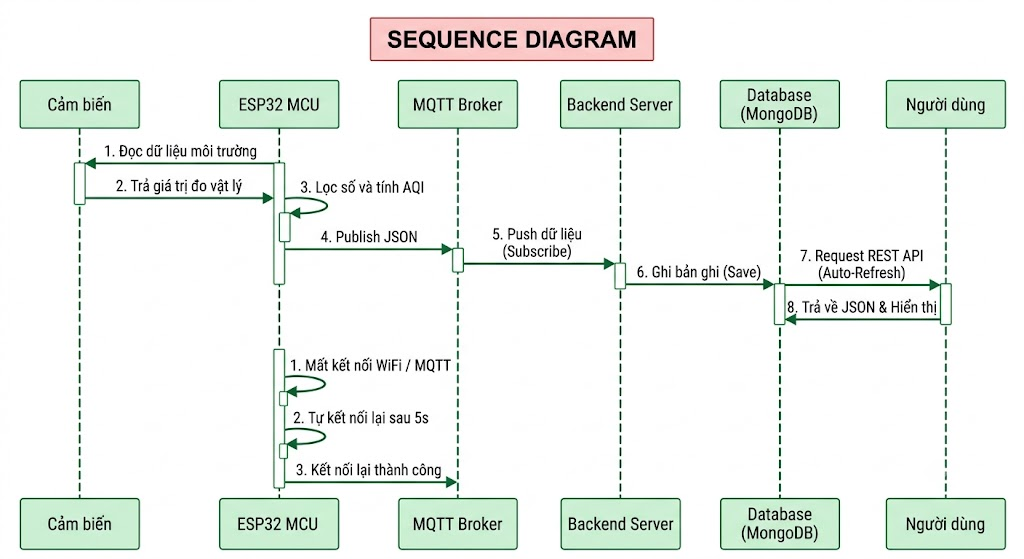
\includegraphics[width=1.0\textwidth]{images/sequence_diagram.png}
    \caption{Biểu đồ tuần tự luồng dữ liệu hệ thống}
    \label{fig:sequence_diagram}
\end{figure}

Biểu đồ mô tả quá trình trao đổi thông tin qua hai kịch bản:
\begin{itemize}
    \item \textbf{Kịch bản 1: Gửi và cập nhật dữ liệu định kỳ}: ESP32 đọc cảm biến $\to$ lọc nhiễu $\to$ tính AQI $\to$ gửi MQTT JSON tới Broker. Backend Subscriber nhận gói tin và ghi vào MongoDB. Trình duyệt người dùng định kỳ gọi API lấy dữ liệu hiển thị lên Dashboard.
    \item \textbf{Kịch bản 2: Kết nối lại khi mất mạng}: Khi mất WiFi hoặc MQTT, ESP32 tự động thử kết nối lại sau mỗi 5 giây.
\end{itemize}

\subsubsection{Thuật toán tổng thể}
Nguyên lý hoạt động tổng thể của hệ thống được thể hiện qua lưu đồ thuật toán chính dưới đây:

\begin{figure}[H]
\centering
\begin{tikzpicture}[node distance=0.5cm,
  block/.style={rectangle, draw, rounded corners=4pt, fill=blue!10, text width=3.5cm, align=center, minimum height=0.85cm, font=\small},
  decision/.style={diamond, draw, fill=orange!15, text width=2.6cm, align=center, aspect=1.8, font=\small},
  wait/.style={rectangle, draw, rounded corners=4pt, fill=gray!15, text width=2.5cm, align=center, minimum height=0.85cm, font=\small},
  arrow/.style={->, >=stealth, thick}]
  \node[block] (boot) {Khởi động ESP32 / Boot};
  \node[block, below=0.5cm of boot] (init) {Khởi tạo ngoại vi};
  \node[decision, below=0.7cm of init] (wifi) {Kết nối\\WiFi/MQTT\\thành công?};
  \node[wait, right=1.6cm of wifi] (retry) {Chờ 5 giây\\Thử kết nối lại};
  \node[block, below=0.7cm of wifi] (read) {Đọc dữ liệu song song};
  \node[block, below=0.5cm of read] (filter) {Áp dụng bộ lọc số};
  \node[block, below=0.5cm of filter] (aqi) {Tính chỉ số AQI\\theo breakpoint US EPA};
  \node[block, below=0.5cm of aqi] (json) {Đóng gói JSON\\(SharedData $\to$ payload)};
  \node[block, below=0.5cm of json] (pub) {Publish MQTT\\tới aqistation/data};
  \node[block, below=0.5cm of pub] (wdt) {Reset Watchdog Timer};
  \node[decision, below=0.7cm of wdt] (alive) {Còn hoạt\\động?};
  \draw[arrow] (boot) -- (init);
  \draw[arrow] (init) -- (wifi);
  \draw[arrow] (wifi) -- node[above, font=\scriptsize]{Không} (retry);
  \draw[arrow] (retry.north) |- (wifi.east);
  \draw[arrow] (wifi) -- node[right, font=\scriptsize]{Có} (read);
  \draw[arrow] (read) -- (filter);
  \draw[arrow] (filter) -- (aqi);
  \draw[arrow] (aqi) -- (json);
  \draw[arrow] (json) -- (pub);
  \draw[arrow] (pub) -- (wdt);
  \draw[arrow] (wdt) -- (alive);
  \draw[arrow] (alive.east) -- ++(0.8,0) |- node[right, font=\scriptsize, pos=0.25]{Có} (read.east);
\end{tikzpicture}
\caption{Lưu đồ thuật toán chính firmware}
\label{fig:main_flowchart}
\end{figure}

\paragraph{Luồng hoạt động tổng thể}\mbox{}\\

\begin{enumerate}
    \item \textbf{Thu thập (Acquisition)}: Ba Task FreeRTOS trên ESP32 đọc song song từ BME680 (I2C), PMS5003 (UART) và MQ-135 (ADC) theo chu kỳ định sẵn. Dữ liệu thô được lưu vào cấu trúc \texttt{SharedData} được bảo vệ bởi Mutex.
    \item \textbf{Lọc nhiễu}: Mỗi cảm biến áp dụng bộ lọc số chuyên biệt:
    \[
    \text{EMA}: \quad x_k = \alpha \cdot r_k + (1-\alpha) \cdot x_{k-1}
    \]
    \[
    \text{Moving Average}: \quad \bar{x}_N = \frac{1}{N}\sum_{i=0}^{N-1} r_{k-i}
    \]
    trong đó $r_k$ là giá trị thô tại thời điểm $k$, $\alpha$ là hệ số làm mượt, $N$ là kích thước cửa sổ.
    \item \textbf{Tính AQI (Computation)}: Sau lọc, ESP32 ánh xạ nồng độ PM2.5, PM10 và MQ-135 lên bảng breakpoint US EPA để tính AQI thành phần, lấy max làm AQI tổng:
    \[
    AQI_p = \left\lfloor \frac{I_{Hi} - I_{Lo}}{C_{Hi} - C_{Lo}} \cdot (C_p - C_{Lo}) + I_{Lo} \right\rceil
    \]
    trong đó $C_p$ là nồng độ đo được, $[C_{Lo}, C_{Hi}]$ và $[I_{Lo}, I_{Hi}]$ là breakpoint nồng độ và AQI tương ứng.
    \item \textbf{Truyền dữ liệu}: \texttt{taskNetwork} serialize \texttt{SharedData} thành chuỗi JSON và publish lên MQTT Broker qua kết nối WiFi 2.4\,GHz. Giao thức MQTT QoS~1 đảm bảo ít nhất một lần giao tin thành công.
    \item \textbf{Tiếp nhận và lưu trữ}: Backend Node.js nhận gói tin, bổ sung timestamp ISO 8601, xác thực cấu trúc JSON và ghi vào MongoDB Atlas.
    \item \textbf{Hiển thị}: Web Dashboard Next.js gọi REST API mỗi 5 giây, nhận dữ liệu JSON từ MongoDB và render biểu đồ, cập nhật các thẻ thông số và kiểm tra ngưỡng cảnh báo.
\end{enumerate}

\subsubsection{Cơ chế xử lý lỗi và tự phục hồi}
\paragraph{Cơ chế chịu lỗi}\mbox{}\\

Hệ thống được thiết kế để xử lý các tình huống mất kết nối mạng:
\begin{itemize}
    \item Khi WiFi mất kết nối, \texttt{taskNetwork} tự động thực hiện Auto-Reconnect sau mỗi 5 giây mà không ảnh hưởng đến các Task đọc cảm biến đang chạy trên Core~1.
    \item Khi kết nối MQTT bị đứt, thư viện PubSubClient tự động kết nối lại với Broker và publish dữ liệu đang chờ trong hàng đợi.
    \item Task Watchdog Timer với ngưỡng 30 giây giám sát mọi Task, tự động reset hệ thống nếu phát hiện Task bị treo (Deadlock).
\end{itemize}

\begin{table}[H]
\centering
\begin{tabular}{|l|l|c|}
\hline
\textbf{Tầng xử lý} & \textbf{Thành phần} & \textbf{Độ trễ tiêu biểu} \\ 
        \hline
Thu thập \& Lọc   & ESP32 + Cảm biến         & $< 100$\,ms \\ 
        \hline
Truyền MQTT        & WiFi + Broker            & 1--5\,giây \\ 
        \hline
Ghi MongoDB        & Backend + Atlas          & 500--2000\,ms \\ 
        \hline
API Response       & Vercel Serverless        & 200--800\,ms \\ 
        \hline
Render Dashboard   & Next.js + Chart.js       & $< 200$\,ms \\ 
        \hline
\textbf{Tổng độ trễ đầu-cuối} & & \textbf{$< 10$\,giây} \\ 
        \hline\end{tabular}
\caption{Tóm tắt luồng dữ liệu và độ trễ tại từng tầng}
\label{tab:latency}

\end{table}

\subsubsection{Quy trình thiết kế và xây dựng dashboard}
Nhằm đảm bảo giao diện giám sát đáp ứng đầy đủ các tiêu chí: trực quan, thời gian thực, có khả năng mở rộng và mang lại trải nghiệm người dùng tối ưu, quy trình thiết kế và phát triển phần mềm giao diện đã được tuân thủ nghiêm ngặt theo mô hình linh hoạt kết hợp với các bước kỹ nghệ phần mềm tiêu chuẩn. Quá trình này được chia thành 5 bước cụ thể và chi tiết như sau:

\noindent\textbf{Bước 1: Phân tích yêu cầu và lên ý tưởng}\mbox{}\\
Trong giai đoạn đầu tiên, nhóm phát triển tiến hành thu thập và phân tích các yêu cầu chức năng cốt lõi mà một hệ thống trạm quan trắc IoT hiện đại cần phải có. 
\begin{itemize}
    \item \textbf{Yêu cầu chức năng:} Người dùng cần xem được ngay lập tức chỉ số AQI tổng hợp và các thông số môi trường (Bụi mịn PM2.5, PM10, Nhiệt độ, Độ ẩm, Áp suất, Nồng độ khí gas). Hệ thống cũng cần có khả năng vẽ biểu đồ theo thời gian để người dùng dễ dàng theo dõi xu hướng, cùng với bản đồ hiển thị vị trí thực tế của trạm đo. Tính năng xác thực tài khoản đăng nhập cũng là một yêu cầu bắt buộc để bảo mật thông tin nội bộ.
    \item \textbf{Yêu cầu phi chức năng:} Độ trễ cập nhật dữ liệu phải thấp (dưới 10 giây). Giao diện phải hoạt động mượt mà trên cả trình duyệt máy tính lẫn thiết bị di động.
\end{itemize}

\noindent\textbf{Bước 2: Lựa chọn công nghệ}\mbox{}\\
Sau khi xác định yêu cầu, nhóm tiến hành đánh giá và lựa chọn các công nghệ phù hợp:
\begin{itemize}
    \item \textbf{Frontend Framework:} Next.js được lựa chọn nhờ khả năng kết hợp hoàn hảo giữa Server-Side Rendering (SSR) và Client-Side Rendering (CSR), giúp tăng tốc độ tải trang ban đầu và tối ưu hóa hệ thống.
    \item \textbf{Styling:} Tailwind CSS được sử dụng để xây dựng giao diện. Hệ thống lớp tiện ích của Tailwind cho phép tùy biến linh hoạt, đồng nhất về thiết kế  và hỗ trợ Mobile-first dễ dàng mà không cần phải viết các tập tin CSS cồng kềnh.
    \item \textbf{Quản lý trạng thái và Biểu đồ:} React Hooks được dùng để quản lý trạng thái dữ liệu thay đổi liên tục. Thư viện \texttt{Chart.js} kết hợp \texttt{react-chartjs-2} được sử dụng để trực quan hóa dữ liệu lịch sử thành các đồ thị đường .
    \item \textbf{Bản đồ:} Thư viện \texttt{Leaflet} kết hợp với Tile Layer của Google Maps để tạo nên bản đồ tương tác hiển thị tọa độ trạm mà không cần các khóa API bảo mật phức tạp.
    \item \textbf{Cơ sở dữ liệu và Xác thực:} MongoDB Atlas được chọn làm cơ sở dữ liệu đám mây (NoSQL) nhờ khả năng lưu trữ linh hoạt luồng dữ liệu IoT dạng chuỗi thời gian. Tính năng phân quyền được giao cho thư viện NextAuth.js xử lý kết hợp mã hóa Bcrypt.
\end{itemize}

\noindent\textbf{Bước 3: Thiết kế UI/UX và kiến trúc hệ thống}.
\begin{itemize}
    \item \textbf{Bố cục trang tổng quan:} Chia thành hai phần chính. Phần đầu ở trên cùng chứa tên trạm, trạng thái kết nối và khối tính toán AQI chính, tích hợp thanh trượt màu sắc theo chuẩn US EPA. Phần dưới hiển thị các thông số phụ chia theo dạng lưới (Grid 2 cột trên điện thoại, 4 cột trên máy tính bàn).
    \item \textbf{Thanh điều hướng:} Hệ thống sử dụng một Sidebar gắn lề trái màn hình, hỗ trợ thu gọn hoặc bung rộng, giúp người dùng dễ dàng chuyển đổi giữa các module: Dashboard, Lịch sử (History), Bản đồ (Map) và Cài đặt (Settings).
    \item \textbf{Thiết kế luồng dữ liệu:} Trình duyệt định kỳ mỗi 10 giây gửi một HTTP GET Request tới REST API \texttt{/api/data/latest} của Next.js Route Handler để lấy dữ liệu từ MongoDB, sau đó cập nhật trực tiếp vào State của React để kích hoạt quá trình Re-render giao diện tự động.
\end{itemize}

\noindent\textbf{Bước 4: Triển khai lập trình phần mềm}\mbox{}\\
Quá trình lập trình được chia nhỏ thành các thành phần độc lập:
\begin{itemize}
    \item \textbf{Xây dựng các component dùng chung:} Lập trình các nút bấm, thẻ dữ liệu, và khối biểu đồ để tái sử dụng xuyên suốt mã nguồn.
    \item \textbf{Trang Đăng nhập/Đăng ký:} Băm mật khẩu người dùng trước khi ghi vào cơ sở dữ liệu. Thiết lập cảnh báo và ràng buộc các thông báo lỗi trên form (ví dụ: Mật khẩu quá ngắn, yêu cầu ít nhất 6 ký tự) để bảo vệ an toàn cho dữ liệu đầu vào.
    \item \textbf{Tích hợp API và vẽ biểu đồ:} Thiết kế thuật toán chuyển đổi mảng dữ liệu. Chuyển đổi nhãn thời gian từ định dạng ISO thành dạng ``giờ:phút'' để hiển thị. 
\end{itemize}

\noindent\textbf{Bước 5: Kiểm thử và triển khai đám mây}
\begin{itemize}
    \item \textbf{Kiểm thử cục bộ:} Chạy hệ thống ở môi trường phát triển (\texttt{localhost}), giả lập luồng gói tin MQTT liên tục gửi từ ESP32 để đánh giá tốc độ cập nhật giao diện người dùng và kiểm tra tính đúng đắn của các biểu tượng màu sắc đánh giá AQI.
    \item \textbf{Tối ưu hóa hiệu năng:} Giảm thiểu tối đa độ trễ bằng cách tách các module nặng (như biểu đồ và bản đồ) ra khỏi chu kỳ làm mới nếu không có sự thay đổi. Các cờ tải (loading flag) được bổ sung để hiển thị hiệu ứng chờ trực quan trong quá trình truy xuất từ cơ sở dữ liệu.
    \item \textbf{Triển khai tự động hóa:} Toàn bộ mã nguồn giao diện frontend và các API phụ trợ được lưu trữ tại GitHub. Nền tảng Vercel được liên kết trực tiếp để cấu hình quy trình triển khai liên tục (CI/CD). Mỗi khi có cập nhật, Vercel tự động biên dịch  và phân phối lên Internet toàn cầu, đảm bảo hệ thống có khả năng mở rộng tự động và phục vụ 24/7 mà không cần đến máy chủ vật lý truyền thống.
\end{itemize}

\newpage


% ============================================================
%  CHƯƠNG 4. THUẬT TOÁN XỬ LÝ TÍN HIỆU
% ============================================================
\newpage
\begin{center}
    \textbf{\Large CHƯƠNG 4. THUẬT TOÁN XỬ LÝ TÍN HIỆU}
\end{center}
\addcontentsline{toc}{section}{CHƯƠNG 4. THUẬT TOÁN XỬ LÝ TÍN HIỆU}
\setcounter{section}{4}
\setcounter{subsection}{0}

\subsection{Bộ lọc số và làm mượt dữ liệu}

\subsubsection{Giới thiệu về các bộ lọc nhiễu}
Trong môi trường thực tế, tín hiệu thu thập từ các cảm biến vật lý luôn chứa các thành phần nhiễu tần số cao phát sinh do nhiễu đường truyền, sự biến động điện áp nguồn cấp hoặc các tác động cơ học tức thời. Để đảm bảo dữ liệu đo đạc ổn định và phản ánh đúng xu hướng thực của môi trường, hệ thống nhúng cần thực hiện lọc nhiễu số trực tiếp tại biên trước khi tính toán các chỉ số chất lượng.

\subsubsection{Nguyên lý hoạt động}
Hệ thống áp dụng 3 thuật toán lọc số chuyên biệt cho từng loại cảm biến:

\paragraph{Bộ lọc trung bình trượt - Cảm biến PMS5003}\mbox{}\\
Bộ lọc hoạt động bằng cách lấy trung bình cộng của $N$ mẫu dữ liệu liên tiếp gần nhất trong một cửa sổ trượt:
\[
\bar{x}_N = \frac{1}{N}\sum_{i=0}^{N-1} r_{k-i}
\]
Trong đó $r_k$ là giá trị đo thô tại thời điểm $k$, $N = 5$ là kích thước cửa sổ lọc được nhóm lựa chọn. Bộ lọc này giúp làm mịn nồng độ bụi mịn PM2.5 và PM10 vốn có đặc tính thay đổi theo dòng khí và dễ bị biến động tức thời.

\paragraph{Bộ lọc trung bình trượt lũy thừa (EMA) - Cảm biến BME680}\mbox{}\\
Bộ lọc EMA gán trọng số giảm dần theo hàm lũy thừa cho các mẫu đo trong quá khứ, giúp phản ứng nhanh hơn với sự thay đổi thực tế của môi trường:
\[
x_k = \alpha \cdot r_k + (1-\alpha) \cdot x_{k-1}
\]
Trong đó $\alpha = 0.1$ là hệ số làm mượt được cấu hình. Hệ số này giúp giữ ổn định cho các thông số biến thiên chậm như nhiệt độ, độ ẩm và áp suất khí quyển.

\paragraph{Bộ lọc trung vị - Cảm biến MQ-135}\mbox{}\\
Bộ lọc trung vị sắp xếp chuỗi mẫu đo trong cửa sổ kích thước $N$ theo thứ tự tăng dần và lấy giá trị ở giữa làm giá trị đại diện:
\[
x_k = \text{median}\{r_{k}, r_{k-1}, \dots, r_{k-N+1}\}
\]
Với kích thước cửa sổ $N = 11$, bộ lọc này triệt tiêu hiệu quả các xung nhiễu gai nhọn (nhấp nhô điện áp ADC) mà không làm suy giảm thời gian phản hồi của cảm biến MQ-135.

\subsubsection{Quy trình lọc theo thời gian thực}
Cả ba bộ lọc số nêu trên đều được triển khai dưới dạng bộ đệm vòng có kích thước cố định bằng $N$, cấp phát tĩnh trong vùng nhớ DRAM của ESP32 để tránh phân mảnh bộ nhớ động khi hệ thống chạy liên tục trong thời gian dài. Mỗi khi có mẫu đo mới từ cảm biến tương ứng, giá trị cũ nhất trong bộ đệm bị ghi đè bởi mẫu mới, sau đó bộ lọc tính toán lại giá trị đầu ra dựa trên toàn bộ cửa sổ hiện tại:
\begin{itemize}
    \item Đối với PMS5003, bộ đệm Moving Average ($N=5$) được cập nhật mỗi khi \texttt{taskPMS} nhận thành công một khung truyền UART hợp lệ (khoảng 1--2 giây/lần tùy tốc độ truyền của cảm biến).
    \item Đối với BME680, bộ lọc EMA chỉ cần lưu duy nhất giá trị đầu ra của lần lọc trước đó ($x_{k-1}$) thay vì toàn bộ cửa sổ mẫu, giúp tiết kiệm đáng kể bộ nhớ so với Moving Average hay Median; giá trị được cập nhật mỗi chu kỳ đọc I2C 10 giây/lần của \texttt{taskSensors}.
    \item Đối với MQ-135, bộ đệm Median ($N=11$) được cập nhật cùng chu kỳ với BME680 (10 giây/lần) do cả hai đều được đọc trong cùng một vòng lặp của \texttt{taskSensors}.
\end{itemize}
Việc lọc số diễn ra hoàn toàn tại biên trước khi dữ liệu được đóng gói JSON và publish lên MQTT Broker, đảm bảo băng thông truyền tải không bị lãng phí bởi các giá trị nhiễu chưa qua xử lý.

\subsubsection{Đánh giá đáp ứng và độ trễ của bộ lọc}
Việc làm mượt tín hiệu bằng các bộ lọc số luôn đánh đổi giữa mức độ triệt nhiễu và độ trễ đáp ứng khi giá trị đo thay đổi đột ngột. Đối với bộ lọc trung bình trượt có cửa sổ kích thước $N$ mẫu đồng trọng số, độ trễ nhóm xấp xỉ:
\[
\tau_{\text{group}} = \frac{N-1}{2} \times T_s
\]
trong đó $T_s$ là chu kỳ lấy mẫu. Với PMS5003 ($N=5$, $T_s \approx 1.5$\,giây), độ trễ nhóm ước tính khoảng $3$\,giây -- vẫn nằm trong giới hạn yêu cầu độ trễ đầu-cuối dưới 10 giây của hệ thống. Đối với bộ lọc EMA, độ trễ nhóm tương đương được xấp xỉ bởi $\tau_{\text{group}} \approx \frac{1-\alpha}{\alpha} \times T_s$; với $\alpha = 0.1$ và $T_s = 10$\,giây, độ trễ nhóm khoảng $90$\,giây -- chấp nhận được vì nhiệt độ và độ ẩm môi trường vốn biến thiên chậm. Bộ lọc trung vị không có độ trễ nhóm cố định theo công thức tuyến tính do bản chất phi tuyến của phép toán sắp xếp, nhưng về thực nghiệm cho thấy thời gian phản hồi tương đương một bộ lọc tuyến tính có cửa sổ bằng $N/2$ mẫu đối với các thay đổi bậc thang (step change).

\subsection{Giải thuật tính toán chỉ số AQI}
Chỉ số chất lượng không khí AQI được tính toán tại thực địa dựa trên thuật toán breakpoint của Cơ quan Bảo vệ Môi trường Hoa Kỳ (US EPA).

\subsubsection{Bụi mịn PM2.5}
Chỉ số AQI đối với bụi mịn PM2.5 được tính theo công thức nội suy tuyến tính:
\[
I_{\text{PM2.5}} = \left\lfloor \frac{I_{Hi} - I_{Lo}}{C_{Hi} - C_{Lo}} \cdot (C_{\text{PM2.5}} - C_{Lo}) + I_{Lo} \right\rceil
\]
Trong đó $C_{\text{PM2.5}}$ là nồng độ bụi sau lọc, các giá trị $[C_{Lo}, C_{Hi}]$ và $[I_{Lo}, I_{Hi}]$ là các điểm breakpoint nồng độ và AQI tương ứng được quy định bởi US EPA.

\subsubsection{Bụi mịn PM10}
Tương tự PM2.5, chỉ số AQI cho bụi PM10 được tính dựa trên các điểm breakpoint nồng độ bụi PM10 tương ứng:
\[
I_{\text{PM10}} = \left\lfloor \frac{I_{Hi} - I_{Lo}}{C_{Hi} - C_{Lo}} \cdot (C_{\text{PM10}} - C_{Lo}) + I_{Lo} \right\rceil
\]

\subsubsection{Khí gas độc hại (MQ-135)}
Nồng độ khí độc đo được từ cảm biến MQ-135 dưới dạng giá trị tương tự (ADC, sau khi qua bộ lọc trung vị) được quy đổi tuyến tính theo từng đoạn sang một thang chỉ số phụ trợ (0--300) để hiển thị riêng lẻ trên Dashboard. Tuy nhiên, chỉ số này \textbf{không} được đưa vào công thức tính AQI tổng hợp của trạm, vì hai lý do kỹ thuật quan trọng:
\begin{itemize}
    \item Giá trị ADC thô của MQ-135 (thường nằm trong khoảng 200--400 khi đo trong không khí sạch tại điều kiện thực nghiệm của nhóm) chưa được hiệu chuẩn (calibrate) theo nồng độ ppm chuẩn bằng khí mẫu tham chiếu, nên không thể quy đổi chính xác sang thang AQI chuẩn US EPA vốn yêu cầu đơn vị nồng độ vật lý xác định.
    \item Qua khảo sát thực nghiệm trên hơn 31.000 bản ghi dữ liệu thu thập được, phần lớn giá trị ADC nền (baseline) của MQ-135 nằm dưới ngưỡng 800, tương ứng chỉ số phụ AQI\_mq luôn nhỏ hơn 50 (mức Tốt); nếu đưa trực tiếp vào phép lấy \texttt{max} sẽ không làm thay đổi kết quả AQI tổng hợp trong hầu hết các trường hợp nhưng lại dễ gây nhiễu cảnh báo giả khi có dao động nền của cảm biến bán dẫn.
\end{itemize}
Giá trị MQ-135 sau lọc vẫn được đóng gói và gửi lên MQTT/Dashboard như một thông số bổ sung mang tính tham khảo, phục vụ người dùng theo dõi xu hướng khí độc cục bộ.

\subsubsection{Tính toán chỉ số AQI tổng hợp}
Do chỉ có PM2.5 và PM10 sở hữu bảng breakpoint chuẩn hóa quốc tế và không đòi hỏi hiệu chuẩn cảm biến bổ sung, chỉ số AQI tổng hợp đại diện cho chất lượng không khí tại trạm đo được nhóm xác định bằng giá trị lớn nhất giữa hai chỉ số thành phần bụi mịn, theo đúng nguyên tắc "chỉ số ô nhiễm chi phối" của US EPA:
\[
AQI_{\text{trạm}} = \max(I_{\text{PM2.5}},\; I_{\text{PM10}})
\]
Chỉ số phụ trợ từ MQ-135 ($I_{\text{Gas}}$) được tính toán và hiển thị song song nhưng \textbf{không} tham gia vào phép lấy \texttt{max} nói trên.

\paragraph{Lưu đồ thuật toán tra bảng breakpoint và tính AQI}\mbox{}\\

Thay vì trình bày đoạn mã tính toán, thuật toán tra cứu breakpoint và nội suy tuyến tính được biểu diễn dưới dạng lưu đồ như sau:

\begin{figure}[H]
\centering
\begin{tikzpicture}[node distance=0.5cm,
  block/.style={rectangle, draw, rounded corners=4pt, fill=blue!10, text width=3.8cm, align=center, minimum height=0.85cm, font=\small},
  decision/.style={diamond, draw, fill=orange!15, text width=2.8cm, align=center, aspect=1.8, font=\small},
  clamp/.style={rectangle, draw, rounded corners=4pt, fill=red!10, text width=2.8cm, align=center, minimum height=0.85cm, font=\small},
  arrow/.style={->, >=stealth, thick}]
  \node[block] (input) {Nồng độ $C_p$ sau lọc\\(PM2.5 hoặc PM10)};
  \node[block, below=0.5cm of input] (scan) {Duyệt bảng breakpoint US EPA\\tìm khoảng $[C_{Lo}, C_{Hi}]$\\chứa $C_p$};
  \node[decision, below=0.7cm of scan] (found) {Tìm thấy\\khoảng\\phù hợp?};
  \node[clamp, right=1.5cm of found] (clamp) {Giới hạn (Clamp)\\về khoảng\\biên gần nhất};
  \node[block, below=0.7cm of found] (interp) {
    Nội suy tuyến tính:\\[4pt]
    $I_p = \dfrac{I_{Hi}-I_{Lo}}{C_{Hi}-C_{Lo}}(C_p - C_{Lo}) + I_{Lo}$
  };
  \node[block, below=0.5cm of interp] (round) {Làm tròn $I_p$\\về số nguyên gần nhất};
  \node[block, below=0.5cm of round] (out) {Trả về chỉ số AQI\\thành phần $I_p$};
  \draw[arrow] (input) -- (scan);
  \draw[arrow] (scan) -- (found);
  \draw[arrow] (found) -- node[above, font=\scriptsize]{Không (ngoài dải)} (clamp);
  \draw[arrow] (clamp.south) -- ++(0,-0.4) -| (interp.east);
  \draw[arrow] (found) -- node[right, font=\scriptsize]{Có} (interp);
  \draw[arrow] (interp) -- (round);
  \draw[arrow] (round) -- (out);
\end{tikzpicture}
\caption{Lưu đồ thuật toán tra bảng breakpoint và nội suy tính chỉ số AQI thành phần}
\label{fig:aqi_flowchart}
\end{figure}

Thuật toán tra bảng breakpoint và nội suy nêu trên được thực thi riêng biệt cho từng thông số bụi mịn PM2.5 và PM10 sau lọc; giá trị MQ-135 được đưa qua một hàm quy đổi tuyến tính từng đoạn riêng để ra chỉ số phụ trợ nhưng không đi qua bảng breakpoint chuẩn US EPA. Cuối cùng, giá trị lớn nhất giữa hai chỉ số thành phần PM2.5 và PM10 được chọn làm chỉ số AQI tổng hợp đại diện cho trạm đo tại thời điểm hiện tại, theo đúng nguyên tắc "chỉ số ô nhiễm chi phối" của chuẩn US EPA.

% ============================================================
%  CHƯƠNG 5. KẾT QUẢ THỰC HIỆN
% ============================================================
\newpage
\begin{center}
    \textbf{\Large CHƯƠNG 5. KẾT QUẢ THỰC HIỆN}
\end{center}
\addcontentsline{toc}{section}{CHƯƠNG 5. KẾT QUẢ THỰC HIỆN}
\setcounter{section}{5}
\setcounter{subsection}{0}

Sau quá trình thiết kế và lập trình, trạm quan trắc chất lượng không khí đã được hoàn thiện cả về phần cứng và ứng dụng giám sát đám mây.

\subsection{Kết quả phần cứng thực tế}

Thiết bị phần cứng hoàn chỉnh được gia công trên mạch in PCB 1 lớp chống nhiễu, bao bọc trong hộp bảo vệ nhựa ABS có khe thông gió tự nhiên để đảm bảo luồng không khí lưu thông tối ưu qua các cảm biến.

\begin{figure}[H]
    \centering
    \textbf{[CHÈN HÌNH ẢNH THỰC TẾ TRẠM QUAN TRẮC VÀO ĐÂY]}
    % \includegraphics[width=0.8\textwidth]{images/hardware_real.png}
    \caption{Hình ảnh thực tế của trạm quan trắc chất lượng không khí}
    \label{fig:hardware_real}
\end{figure}

Khối sensor bao gồm toàn bộ các thiết bị cảm biến vật lý có nhiệm vụ đo lường trực tiếp các thông số môi trường không khí. Đây là nguồn dữ liệu đầu vào duy nhất của hệ thống.

\begin{table}[H]
\centering
\caption{Danh sách cảm biến trong hệ thống và thông số đo}
\label{tab:sensor_block}
\begin{tabularx}{\textwidth}{|l|l|>{\raggedright\arraybackslash}X|}
\hline
\textbf{Cảm biến} & \textbf{Giao tiếp} & \textbf{Thông số đo} \\ 
\hline
BME680  & I2C (tự động quét 0x76/0x77) & Nhiệt độ ($-40 \div 85^\circ$C, đã bù trừ tự phát nhiệt), Độ ẩm (0--100\%RH), Áp suất (300--1100\,hPa), Điện trở khí VOC \\ 
\hline
PMS5003 & UART2, 9600 baud & PM1.0, PM2.5, PM10 (0--500\,$\mu$g/m$^3$); số hạt theo 6 dải kích thước \\ 
\hline
MQ-135  & ADC1 (GPIO34) & Tín hiệu tương tự 0--3.3\,V, chuyển đổi sang nồng độ ppm (NH$_3$, CO$_2$, VOC) \\ 
\hline
\end{tabularx}
\end{table}

Ba cảm biến này hoạt động song song và bổ sung cho nhau để tạo ra bức tranh toàn diện về chất lượng không khí:
\begin{itemize}
    \item \textbf{BME680} cung cấp thông số vi khí hậu (nhiệt độ, độ ẩm, áp suất) -- vừa là dữ liệu đo trực tiếp, vừa làm tham chiếu để bù sai số nhiệt-ẩm cho MQ-135.
    \item \textbf{PMS5003} chuyên đo nồng độ hạt bụi lơ lửng với độ chính xác cao bằng công nghệ tán xạ laser -- đây là thông số quan trọng nhất trong tính toán AQI.
    \item \textbf{MQ-135} phản ánh tổng hợp chất lượng không khí qua điện trở bán dẫn $\text{SnO}_2$ -- nhạy cảm với các khí độc hại như NH$_3$, CO và các hợp chất hữu cơ bay hơi.
\end{itemize}

\begin{figure}[H]
    \centering
    \textbf{[CHÈN HÌNH ẢNH THỰC TẾ CHI TIẾT CÁC CẢM BIẾN VÀO ĐÂY]}
    % \includegraphics[width=0.8\textwidth]{images/sensors_real.png}
    \caption{Các module cảm biến được tích hợp bên trong trạm đo}
    \label{fig:sensors_real}
\end{figure}

\subsection{Kết quả phần mềm backend và cơ sở dữ liệu MongoDB}
Hệ thống lưu trữ cơ sở dữ liệu MongoDB Atlas hoạt động ổn định. Khối server là tầng trung gian đảm nhận việc tiếp nhận, xử lý và lưu trữ dữ liệu từ ESP32, đồng thời cung cấp API cho giao diện web. Hệ thống sử dụng kiến trúc backend serverless trên nền tảng Vercel kết hợp cơ sở dữ liệu MongoDB Atlas.

\paragraph{MQTT Subscriber}\mbox{}\\
Dịch vụ Node.js chạy liên tục, kết nối bất đồng bộ đến MQTT Broker công cộng \texttt{broker.emqx.io} qua cổng 1883, lắng nghe topic \texttt{aqistation/data}. Khi nhận được gói tin, hệ thống parse JSON, bổ sung \texttt{timestamp} và ghi bản ghi vào MongoDB.

\subsubsection{Cơ sở dữ liệu MongoDB Atlas}
\paragraph{Ví dụ bản ghi thực tế}\mbox{}\\
Dưới đây là một bản ghi JSON mẫu trích xuất thực tế từ MongoDB Client khi thiết bị thực hiện đo lường và đẩy dữ liệu lên cơ sở dữ liệu:
\begin{lstlisting}[language=json, basicstyle=\footnotesize\ttfamily, backgroundcolor=\color{gray!10}, frame=single]
{
  "_id": "64bc1a2f9d3e4a1b2c3d4e5f",
  "pm2_5": 35.2,
  "pm10": 42.1,
  "temperature": 32.5,
  "humidity": 68.4,
  "pressure": 1005,
  "gas_resistance": 45,
  "aqi": 99,
  "timestamp": "2023-07-22T10:15:30.000Z",
  "__v": 0
}
\end{lstlisting}

\paragraph{Lý do lựa chọn}\mbox{}\\
Dự án quyết định lựa chọn cơ sở dữ liệu phi quan hệ (NoSQL) MongoDB thay vì các hệ quản trị CSDL quan hệ (SQL) truyền thống dựa trên các đặc thù của dữ liệu IoT:
\begin{itemize}
    \item \textbf{Đặc thù dữ liệu Time-Series:} Dữ liệu quan trắc từ trạm IoT liên tục được ghi mới theo chu kỳ ngắn (ghi nhiều) và thường được truy vấn theo khoảng thời gian để vẽ biểu đồ (đọc theo khoảng thời gian). MongoDB tối ưu hóa rất tốt cho kiểu dữ liệu Time-Series này thông qua việc đánh chỉ mục (Index) trường \texttt{timestamp}.
    \item \textbf{Schema linh hoạt (Flexible Schema):} Dữ liệu từ cảm biến gửi lên dưới dạng JSON. MongoDB lưu trữ dữ liệu dưới định dạng BSON (tương tự JSON), giúp việc ánh xạ (mapping) trực tiếp từ payload MQTT sang Database diễn ra tự nhiên, không cần định nghĩa các bảng ghép nối phức tạp.
    \item \textbf{Hiệu năng nạp dữ liệu (Write Performance):} MongoDB hỗ trợ ghi dữ liệu tốc độ cao, hoàn toàn phù hợp với luồng dữ liệu thời gian thực không ngừng nghỉ từ thiết bị nhúng.
\end{itemize}

\subsubsection{Mô tả REST API}

\paragraph{Bảng endpoint}\mbox{}\\
Hệ thống Backend (Next.js API Routes) cung cấp các REST API sau nhằm phục vụ giao diện hiển thị:

\begin{table}[H]
\centering
\caption{Danh sách REST API endpoint của hệ thống}
\label{tab:rest_api}
\begin{tabularx}{\textwidth}{|l|l|>{\raggedright\arraybackslash}X|l|>{\raggedright\arraybackslash}X|}
\hline
\textbf{Method} & \textbf{URL} & \textbf{Chức năng} & \textbf{Tham số đầu vào} & \textbf{Ví dụ response JSON} \\ 
\hline
GET & \texttt{/api/data/latest} & Lấy bản ghi đo môi trường mới nhất & Không có & \texttt{\{"pm2\_5\":35,"aqi":99,...\}} \\ 
\hline
GET & \texttt{/api/data} & Lấy danh sách lịch sử đo theo số lượng & \texttt{?limit=60} (số bản ghi) & \texttt{[\{"pm2\_5\":35\}, \{"pm2\_5\":36\}]} \\ 
\hline
POST & \texttt{/api/alert/check} & Kích hoạt kiểm tra thông số vượt ngưỡng cảnh báo & Không có & \texttt{\{"alert\": true, "msg": "..."\}} \\ 
\hline
\end{tabularx}
\end{table}

\paragraph{Ví dụ thực tế}\mbox{}\\
Dưới đây là mô phỏng Request và Response thực tế cho endpoint quan trọng nhất lấy lịch sử dữ liệu (sử dụng lệnh cURL):

\textbf{Request:}
\begin{lstlisting}[language=bash, basicstyle=\footnotesize\ttfamily, backgroundcolor=\color{gray!10}, frame=single]
curl -X GET "https://aqistation.vercel.app/api/data?limit=2"
\end{lstlisting}

\textbf{Response (Status 200 OK):}
\begin{lstlisting}[language=json, basicstyle=\footnotesize\ttfamily, backgroundcolor=\color{gray!10}, frame=single]
[
  {
    "_id": "64bc1a2f9d...",
    "pm2_5": 35.2,
    "temperature": 32.5,
    "aqi": 99,
    "timestamp": "2023-07-22T10:15:30.000Z"
  },
  {
    "_id": "64bc1a3f9d...",
    "pm2_5": 36.1,
    "temperature": 32.6,
    "aqi": 102,
    "timestamp": "2023-07-22T10:15:35.000Z"
  }
]
\end{lstlisting}

\paragraph{Xác thực (Authentication)}\mbox{}\\
\begin{itemize}
    \item \textbf{Cơ chế bảo vệ trang quản trị Dashboard:} Hệ thống hiện tại áp dụng cơ chế xác thực dựa trên thư viện NextAuth.js kết nối với cơ sở dữ liệu MongoDB (collection \texttt{users}). Quá trình đăng nhập trả về một Session Token (được mã hóa JWT và lưu trong cookie an toàn của trình duyệt), đảm bảo chỉ những tài khoản hợp lệ mới có thể truy cập các trang nội bộ của Web Dashboard.
    \item \textbf{Với các public REST API lấy dữ liệu (\texttt{/api/data...}):} Hiện tại, các endpoint đọc dữ liệu cảm biến được thiết kế ở trạng thái "Mở" (Public) không yêu cầu xác thực. \textit{Lý do:} Mục đích của trạm quan trắc là chia sẻ thông tin chất lượng không khí cộng đồng nên việc đọc dữ liệu là công khai. Tuy nhiên, luồng ghi dữ liệu từ MQTT Subscriber vào MongoDB đã được che giấu ở tầng server-side (ẩn hoàn toàn khỏi Client).
    \item \textbf{Phương án triển khai thực tế tương lai:} Khi phát triển mở rộng cho phép bên thứ 3 lấy dữ liệu, hệ thống sẽ áp dụng \textbf{API Key} được cấp phát riêng cho từng đối tác. Client sẽ cần truyền Key qua HTTP Header (ví dụ: \texttt{Authorization: Bearer <API\_KEY>}) để Backend kiểm soát lưu lượng truy cập (Rate Limiting).
\end{itemize}

\subsection{Kết quả hiển thị Web Dashboard}
Để người dùng có thể dễ dàng theo dõi và tương tác với dữ liệu từ hệ thống, nhóm đã xây dựng một Web Dashboard trực quan sử dụng framework Next.js kết hợp với Chart.js và Tailwind CSS. Giao diện được triển khai trên nền tảng Vercel, đảm bảo khả năng truy cập linh hoạt từ mọi thiết bị có trình duyệt (máy tính, điện thoại, máy tính bảng) mọi lúc, mọi nơi.

\subsubsection{Hiển thị chỉ số AQI và cảnh báo màu sắc}
Trung tâm của trang Dashboard là bảng hiển thị chỉ số AQI tổng hợp theo thời gian thực. Giá trị AQI được hiển thị nổi bật kèm nhãn phân loại tự động và thanh trượt dải màu tuyến tính theo chuẩn US EPA. Card AQI có màu nền động thay đổi theo mức độ cảnh báo, giúp người dùng dễ dàng nhận diện các thông số bất thường chỉ bằng một cái nhìn:

\begin{table}[H]
\centering
\caption{Thang phân loại AQI và màu cảnh báo theo chuẩn US EPA}
\label{tab:aqi_levels}
\begin{tabular}{|c|l|l|}
\hline
\textbf{Dải AQI} & \textbf{Phân loại} & \textbf{Màu hiển thị} \\
\hline
0 -- 50   & Tốt                          & Xanh lá  \\
\hline
51 -- 100  & Trung bình                   & Vàng     \\
\hline
101 -- 150 & Không tốt cho nhóm nhạy cảm & Cam      \\
\hline
151 -- 200 & Không tốt                    & Đỏ       \\
\hline
201 -- 300 & Rất xấu                      & Tím      \\
\hline
301 -- 500 & Nguy hại                     & Nâu đỏ   \\
\hline
\end{tabular}
\end{table}

\begin{figure}[H]
    \centering
    % \includegraphics[width=1.0\textwidth]{images/dashboard_home.png}
    \fbox{\parbox{0.95\textwidth}{\centering\vspace{2cm}\textit{[Hình ảnh giao diện trang Tổng quan Dashboard -- bổ sung sau]}\vspace{2cm}}}
    \caption{Giao diện trang Tổng quan với chỉ số AQI, thanh màu US EPA và thẻ thông số}
    \label{fig:dashboard_top}
\end{figure}

\subsubsection{Hiển thị các thông số môi trường chi tiết}

Dashboard hiển thị 4 thẻ thông số (card) cốt lõi với icon trực quan ngay bên dưới bảng AQI:
\begin{itemize}
    \item Nhiệt độ (°C) -- Icon nhiệt kế
    \item Độ ẩm (\%) -- Icon giọt nước
    \item Mức Gas (ppm) -- Icon khí độc
    \item Mật độ bụi ($\mu$g/m\textsuperscript{3}) -- Icon bụi mịn
\end{itemize}

Mỗi thẻ được thiết kế tối giản, tập trung làm nổi bật giá trị số đo kèm đơn vị. Thanh trạng thái hệ thống ở góc trên cùng hiển thị tên trạm, thời điểm cập nhật gần nhất và chỉ báo \textbf{Trực tuyến/Ngoại tuyến} sử dụng hiệu ứng nhấp nháy (pulse).

\begin{figure}[H]
    \centering
    % \includegraphics[width=1.0\textwidth]{images/dashboard_cards.png}
    \fbox{\parbox{0.95\textwidth}{\centering\vspace{2cm}\textit{[Hình ảnh các thẻ thông số môi trường -- bổ sung sau]}\vspace{2cm}}}
    \caption{Các thông số môi trường hiển thị dạng card với icon trực quan}
    \label{fig:dashboard_cards}
\end{figure}

\subsubsection{Biểu đồ lịch sử AQI theo thời gian}

Hệ thống sử dụng Chart.js để vẽ các biểu đồ tương tác. Hệ thống vẽ đồng thời 6 biểu đồ đường (Line Chart) diễn biến theo thời gian thực cho toàn bộ các thông số: PM2.5, PM10, Nhiệt độ, Độ ẩm, Áp suất và Gas VOC. Menu thả xuống cho phép người dùng tùy chọn khung thời gian xem linh hoạt (1 phút, 5 phút, 1 giờ, 24 giờ).

Tính năng này cho phép người dùng:
\begin{itemize}
    \item Theo dõi xu hướng thay đổi của chất lượng không khí trong 24 giờ qua
    \item Xác định các thời điểm ô nhiễm cao điểm trong ngày
    \item Phân tích mối liên hệ giữa các yếu tố môi trường
    \item Có cơ sở để lên kế hoạch và điều chỉnh các hoạt động cho phù hợp
\end{itemize}

\begin{figure}[H]
    \centering
    % 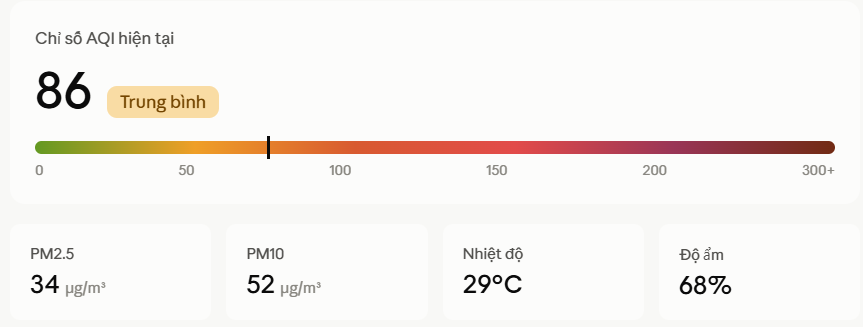
\includegraphics[width=1.0\textwidth]{images/dashboard_charts.png}
    \fbox{\parbox{0.95\textwidth}{\centering\vspace{2cm}\textit{[Hình ảnh biểu đồ AQI và Nhiệt độ \& Độ ẩm theo thời gian -- bổ sung sau]}\vspace{2cm}}}
    \caption{Biểu đồ lịch sử AQI và các thông số môi trường theo thời gian thực}
    \label{fig:dashboard_charts}
\end{figure}

\subsubsection{Bảng dữ liệu chi tiết}

Một bảng dữ liệu (Data Table) hiển thị 10 bản ghi gần nhất với đầy đủ thông tin:
\begin{itemize}
    \item Timestamp (Thời gian ghi nhận)
    \item Tất cả các thông số cảm biến (Nhiệt độ, Độ ẩm, Gas, Bụi)
    \item Chỉ số AQI với màu sắc phân loại
\end{itemize}

Bảng có khả năng cuộn ngang trên mobile, đảm bảo hiển thị tốt trên mọi kích thước màn hình. Trang Lịch sử cũng cung cấp khối thống kê tổng hợp: Tổng số bản ghi, AQI trung bình, AQI cao nhất và PM2.5 trung bình.

\begin{figure}[H]
    \centering
    % 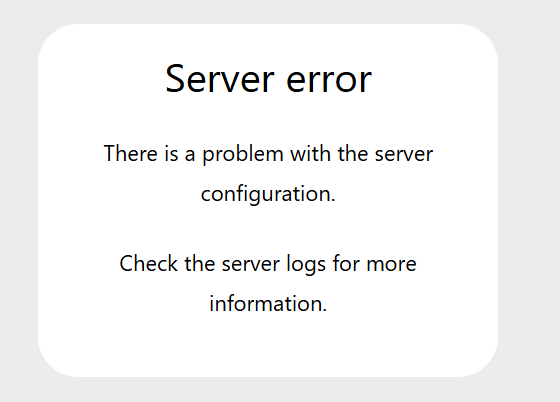
\includegraphics[width=1.0\textwidth]{images/history_table.png}
    \fbox{\parbox{0.95\textwidth}{\centering\vspace{2cm}\textit{[Hình ảnh bảng dữ liệu gần đây -- bổ sung sau]}\vspace{2cm}}}
    \caption{Bảng dữ liệu chi tiết các bản ghi đo theo thời gian}
    \label{fig:history_table}
\end{figure}

\subsubsection{Cập nhật dữ liệu tự động}

\textbf{Auto-refresh:} Dashboard tự động làm mới dữ liệu mỗi 5 giây để đảm bảo hiển thị thông tin mới nhất từ ESP32.

\textbf{Real-time indicator:} Hiển thị thời gian cập nhật gần nhất và trạng thái kết nối thiết bị (dấu chấm xanh nhấp nháy khi trực tuyến, đỏ khi ngoại tuyến).

\textbf{Kiến trúc REST API:} Hệ thống cung cấp các API endpoint chuẩn RESTful để giao tiếp:
\begin{itemize}
    \item \texttt{GET /api/data/latest} \quad -- Lấy bản ghi đo mới nhất
    \item \texttt{GET /api/data/history} \quad -- Lấy lịch sử theo khoảng thời gian
    \item \texttt{GET /api/data/stats} \quad\quad -- Thống kê trung bình theo giờ/ngày
\end{itemize}

\textbf{Hệ thống cảnh báo tùy chỉnh:} Trang Cài đặt cho phép người dùng cấu hình ngưỡng AQI kích hoạt cảnh báo, nhập địa chỉ email nhận thông báo và bật/tắt thông báo Push trực tiếp trên trình duyệt.

\begin{figure}[H]
    \centering
    % 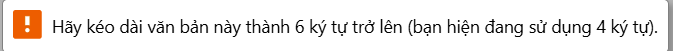
\includegraphics[width=0.95\textwidth]{images/settings_page.png}
    \fbox{\parbox{0.95\textwidth}{\centering\vspace{2cm}\textit{[Hình ảnh giao diện Cài đặt cảnh báo -- bổ sung sau]}\vspace{2cm}}}
    \caption{Giao diện Cài đặt cảnh báo với ngưỡng AQI tùy chỉnh}
    \label{fig:settings_page}
\end{figure}

\subsection{Kết quả kiểm thử các kịch bản thực tế}
Dưới đây là kết quả kiểm chứng chi tiết thông qua các bài test thực nghiệm tại hiện trường:
Để đánh giá tính ổn định, độ nhạy và khả năng tự phục hồi của trạm quan trắc chất lượng không khí, nhóm phát triển đã tiến hành xây dựng và thực hiện 4 kịch bản kiểm thử (Test Cases) thực tế như sau:

\paragraph{Kịch bản 1: Kiểm thử độ nhạy và giải thuật lọc nhiễu đo bụi mịn (PMS5003)}\mbox{}\\
\begin{itemize}
    \item \textbf{Mục tiêu}: Xác thực tốc độ phản hồi và độ mịn của giá trị đo bụi sau khi đi qua bộ lọc Moving Average (cửa sổ $N=5$).
    \item \textbf{Phương pháp thực hiện}: Sử dụng một nguồn khói nhân tạo (đốt nhang) cách cảm biến 15\,cm trong phòng kín khí. Tiến hành kích thích khói trong 60 giây và dập tắt.
    \item \textbf{Kết quả ghi nhận}: Cảm biến PMS5003 phát hiện nồng độ bụi PM2.5 tăng vọt từ mức nền $12\,\mu\text{g/m}^3$ lên đỉnh điểm $150\,\mu\text{g/m}^3$ chỉ sau 3 giây. Đồ thị số liệu trơn tru, không xuất hiện các giá trị ảo đột biến nhờ có bộ lọc trung bình trượt làm mượt tín hiệu.
\end{itemize}

\paragraph{Kịch bản 2: Kiểm thử cảm biến khí độc (MQ-135) và thuật toán Median Filter}\mbox{}\\
\begin{itemize}
    \item \textbf{Mục tiêu}: Xác định khả năng loại bỏ gai nhiễu điện áp tức thời từ cổng ADC1 vi điều khiển.
    \item \textbf{Phương pháp thực hiện}: Sử dụng bật lửa gas (butane) xả nhẹ khí gần buồng đo của MQ-135. Đồng thời tạo ra các xung nhiễu điện bằng cách bật/tắt các thiết bị công suất lớn cạnh nguồn cấp.
    \item \textbf{Kết quả ghi nhận}: Điện áp ADC1 tăng nhanh tương ứng với nồng độ gas tăng. Bộ lọc trung vị (Median Filter, cửa sổ $N=11$) đã triệt tiêu hoàn toàn các xung nhiễu gai nhọn (nhỏ hơn 1 giây) phát sinh khi đóng ngắt tải điện, đảm bảo giá trị MQ-135 gửi lên server phản ánh đúng thực tế.
\end{itemize}

\paragraph{Kịch bản 3: Thử nghiệm khả năng chịu lỗi truyền thông WiFi và MQTT}\mbox{}\\
\begin{itemize}
    \item \textbf{Mục tiêu}: Đảm bảo tiến trình kết nối lại hoạt động độc lập và không gây nghẽn hệ thống.
    \item \textbf{Phương pháp thực hiện}: Tiến hành ngắt kết nối nguồn của bộ phát sóng WiFi (Access Point) trong thời gian 5 phút khi hệ thống đang hoạt động bình thường, sau đó bật lại nguồn phát.
    \item \textbf{Kết quả ghi nhận}: Task truyền mạng \texttt{taskNetwork} trên Core 0 phát hiện mất kết nối sau 15 giây, tự động rơi vào chu kỳ quét kết nối lại mỗi 5 giây mà không làm gián đoạn hai task đọc cảm biến (\texttt{taskPMS} và \texttt{taskSensors}) đang thực thi độc lập trên Core 1. Khi WiFi hoạt động trở lại, kết nối MQTT tự khôi phục thành công và dữ liệu lại được publish bình thường.
\end{itemize}

\paragraph{Kịch bản 4: Kiểm thử bộ giám sát tự động bằng Watchdog Timer}\mbox{}\\
\begin{itemize}
    \item \textbf{Mục tiêu}: Kiểm tra khả năng tự khởi động lại phần cứng của ESP32 khi xảy ra lỗi treo phần mềm.
    \item \textbf{Phương pháp thực hiện}: Cài đặt một đoạn mã thử nghiệm tạo vòng lặp vô hạn nhân tạo bên trong \texttt{taskSensors} để khóa hoàn toàn quyền điều phối của nhân CPU 1.
    \item \textbf{Kết quả ghi nhận}: Tác vụ bị treo dẫn đến hàm xóa watchdog \texttt{esp\_task\_wdt\_reset()} không được gọi. Sau đúng 30 giây (định mức cấu hình \texttt{WDT\_TIMEOUT\_S}), phần cứng Watchdog phát hiện vi phạm và tự động kích hoạt ngắt Reset cứng hệ thống, thiết bị tự khởi động lại và khôi phục trạng thái hoạt động bình thường thành công.
\end{itemize}

% ============================================================
%  KẾT LUẬN VÀ HƯỚNG PHÁT TRIỂN
% ============================================================
\newpage
\begin{center}
    \textbf{\Large KẾT LUẬN}
\end{center}
\addcontentsline{toc}{section}{KẾT LUẬN}

\paragraph*{Kết luận}\mbox{}\\
Dự án đã hoàn thành xuất sắc mục tiêu chế tạo một trạm quan trắc không khí IoT toàn diện, kết hợp hài hòa giữa phần cứng nhúng biên và hạ tầng kỹ thuật phần mềm hiện đại. Những thành tựu cốt lõi có thể tóm lược như sau:
\begin{itemize}
    \item Thiết kế và gia công thành công bo mạch PCB với cấu trúc nguồn điện phân ly chống nhiễu, tích hợp gọn gàng cảm biến hạt lơ lửng PMS5003, cảm biến khí hậu BME680, khí MQ-135 và màn hình cảnh báo OLED cục bộ.
    \item Tối ưu hóa sâu sắc kiến trúc lập trình đa luồng trên hệ điều hành FreeRTOS, triển khai thuật toán tính toán AQI chuẩn xác theo US EPA và các bộ lọc số triệt tiêu nhiễu phần cứng.
    \item Xây dựng một đường ống dữ liệu hoàn chỉnh: từ giao thức MQTT siêu nhẹ ở tầng kết nối, cơ sở dữ liệu Time-Series MongoDB tốc độ cao, đến giao diện hiển thị Next.js mượt mà được vận hành trên hạ tầng đám mây phân tán Vercel.
\end{itemize}

\paragraph*{Hướng phát triển tương lai}\mbox{}\\
Dù đáp ứng tốt các chỉ tiêu kỹ thuật, hệ thống vẫn tồn tại điểm yếu chí mạng khi bị ngắt kết nối mạng Internet (Blackout) diện rộng do không lưu trữ đệm dữ liệu. Trong giai đoạn tiếp theo, hệ thống sẽ được nghiên cứu nâng cấp ở các hạng mục:
\begin{enumerate}
    \item \textbf{Cơ chế lưu trữ đệm:} Tận dụng phân vùng nhớ Flash nội bộ của ESP32 (thông qua chuẩn SPIFFS hoặc LittleFS) để lưu các gói tin JSON khi rớt mạng, tự động đẩy bù đồng loạt khi có mạng trở lại.
    \item \textbf{Hệ thống năng lượng xanh tự chủ:} Thiết kế thêm mạch quản lý sạc năng lượng mặt trời kết hợp kích hoạt chế độ ngủ sâu trên lõi ESP32, cho phép trạm được triển khai độc lập ở các khu vực hẻo lánh, công viên ngoài trời mà không cần lưới điện 220V.
    \item \textbf{Học máy cảnh báo sớm:} Thu thập dữ liệu trên quy mô năm và huấn luyện các mô hình dự báo chuỗi thời gian để cảnh báo trước các đợt không khí xấu, tích hợp tính năng gửi tin nhắn Telegram/Email tự động đến người dân trong khu vực.
\end{enumerate}

\newpage

\newpage
% ============================================================
%  TÀI LIỆU THAM KHẢO
% ============================================================
\begin{thebibliography}{99}

\bibitem{epa2018aqi}
U.S. Environmental Protection Agency,
\emph{Technical Assistance Document for the Reporting of Daily Air Quality -- the Air Quality Index (AQI)}.
EPA 454/B-18-007, 2018.

\bibitem{espressif2023}
Espressif Systems,
\emph{ESP32 Series Datasheet}, v4.1.
Espressif Systems, 2023.

\bibitem{mqtt2014}
OASIS Standard,
\emph{MQTT Version 3.1.1}.
\url{http://docs.oasis-open.org/mqtt/mqtt/v3.1.1/os/mqtt-v3.1.1-os.html}, 2014.

\bibitem{bosch2018bme680}
Bosch Sensortec,
\emph{BME680 Datasheet -- Environmental sensor}.
BST-BME680-DS001, 2018.

\bibitem{plantower2016pms5003}
Plantower Co., Ltd.,
\emph{PMS5003 Particulate Matter Sensor Datasheet}.
2016.

\bibitem{barry2016freertos}
Richard Barry,
\emph{Mastering the FreeRTOS Real Time Kernel -- A Hands On Tutorial Guide}.
FreeRTOS.org, 2016.

\bibitem{oppenheim2009dsp}
A.~V. Oppenheim and R.~W. Schafer,
\emph{Discrete-Time Signal Processing}, 3rd ed.
Prentice Hall, 2009.

\end{thebibliography}




\newpage
% ============================================================
%  PHỤ LỤC
% ============================================================
\begin{center}
    \textbf{\Large PHỤ LỤC}
\end{center}
\addcontentsline{toc}{section}{PHỤ LỤC}
\renewcommand{\thesubsection}{\Alph{subsection}.}
\renewcommand{\thesubsubsection}{\Alph{subsection}.\arabic{subsubsection}}
\renewcommand{\theparagraph}{\Alph{subsection}.\arabic{subsubsection}.\arabic{paragraph}}
\renewcommand{\thesubparagraph}{\Alph{subparagraph}.}
\setcounter{subsection}{0}


\subsection{Giới thiệu chi tiết về các thông số môi trường đo đạc}

\subsubsection{Bụi mịn PM2.5 và PM10}
Bụi mịn là hỗn hợp các hạt rắn và giọt lỏng lơ lửng trong không khí, được phân loại theo đường kính khí động học. PM10 bao gồm các hạt có đường kính nhỏ hơn hoặc bằng $10\,\mu\text{m}$, có thể xâm nhập vào đường hô hấp trên. PM2.5 -- các hạt có đường kính nhỏ hơn hoặc bằng $2.5\,\mu\text{m}$ -- nguy hiểm hơn nhiều vì có khả năng xâm nhập sâu vào phế nang phổi và thậm chí đi vào máu, gây ra các bệnh lý tim mạch và hô hấp mãn tính. Nguồn phát thải chính của bụi mịn tại đô thị Việt Nam bao gồm khí thải giao thông, hoạt động xây dựng, đốt rác thải và nấu nướng bằng nhiên liệu rắn.

\subsubsection{Các khí độc hại trong không khí (MQ-135)}
Bên cạnh bụi mịn, một số khí độc hại phổ biến ảnh hưởng đến chất lượng không khí đô thị bao gồm:
\begin{itemize}
    \item \textbf{Amoniac (NH$_3$)}: Phát sinh từ chất thải sinh hoạt, chăn nuôi, gây kích ứng đường hô hấp ở nồng độ cao.
    \item \textbf{Carbon monoxide (CO)}: Sinh ra từ quá trình đốt cháy không hoàn toàn (bếp gas, động cơ đốt trong), là khí không màu không mùi nhưng có thể gây ngộ độc nghiêm trọng do cạnh tranh với oxy trong máu.
    \item \textbf{Hợp chất hữu cơ bay hơi (VOC)}: Phát sinh từ sơn, dung môi, khói thuốc lá, có thể gây kích ứng và về lâu dài ảnh hưởng đến gan, thận, hệ thần kinh.
\end{itemize}

\subsubsection{Các chỉ số vi khí hậu (Nhiệt độ, Độ ẩm, Áp suất từ BME680)}
Nhiệt độ, độ ẩm và áp suất khí quyển đóng vai trò quan trọng trong việc phản ánh trạng thái của khí quyển:
\begin{itemize}
    \item \textbf{Nhiệt độ}: Ảnh hưởng đến tốc độ khuếch tán và động học của các phân tử khí.
    \item \textbf{Độ ẩm}: Độ ẩm cao thúc đẩy sự ngưng tụ của các hạt bụi mịn, làm tăng kích thước động học của chúng và ảnh hưởng trực tiếp đến phép đo quang học của cảm biến PMS5003.
    \item \textbf{Áp suất khí quyển}: Phản ánh sự đối lưu không khí, áp suất thấp thường đi kèm với hiện tượng nghịch nhiệt, tích tụ chất ô nhiễm sát mặt đất.
\end{itemize}

\subsubsection{Mối liên hệ vật lý giữa bụi mịn, khí độc và vi khí hậu}
Sự kết hợp giữa vi khí hậu và chất ô nhiễm tạo ra các kịch bản môi trường phức tạp:
\begin{itemize}
    \item Trong những ngày nhiệt độ cao và độ ẩm thấp, bụi mịn dễ bị phát tán và lơ lửng lâu hơn trong không khí.
    \item Độ ẩm cao khiến các hạt bụi mịn hấp thụ hơi nước và tăng trọng lượng, dễ bị lắng đọng nhưng cũng dễ bám dính vào màng lọc cảm biến gây sai số.
    \item Sự thay đổi nhiệt độ ảnh hưởng trực tiếp đến điện trở lớp nhạy khí oxit kim loại của cảm biến MQ-135, đòi hỏi thuật toán bù trừ nhiệt-ẩm từ cảm biến BME680 để đảm bảo tính ổn định của phép đo nồng độ khí độc.
\end{itemize}

\subsubsection{Chỉ số chất lượng không khí AQI}
Chỉ số AQI (Air Quality Index) là một thang đo không thứ nguyên được US EPA phát triển nhằm quy đổi nồng độ các chất ô nhiễm khác nhau về một thang điểm chung dễ hiểu (0--500), giúp công chúng dễ dàng đánh giá mức độ ô nhiễm và nguy cơ sức khỏe tương ứng mà không cần hiểu các đơn vị đo chuyên môn ($\mu\text{g/m}^3$, ppm...). Thang AQI được chia thành 6 mức cảnh báo màu sắc như đã trình bày ở Bảng~\ref{tab:aqi_levels}, mỗi mức tương ứng với khuyến cáo sức khỏe cụ thể cho cả người khỏe mạnh và nhóm nhạy cảm (trẻ em, người già, người có bệnh lý hô hấp/tim mạch).

\subsection{Giới thiệu toán học về các bộ lọc số}

\subsubsection{Bộ lọc trung bình trượt}
Bộ lọc hoạt động bằng cách lấy trung bình cộng của $N$ mẫu dữ liệu liên tiếp gần nhất trong một cửa sổ trượt. Phương trình sai phân trong miền thời gian là:
\[
\bar{x}_k = \frac{1}{N}\sum_{i=0}^{N-1} r_{k-i}
\]
Trong đó $r_k$ là giá trị đo thô tại thời điểm $k$, $N = 5$ là kích thước cửa sổ lọc.

\subsubsection{Bộ lọc trung bình trượt lũy thừa}
Bộ lọc EMA gán trọng số giảm dần theo hàm lũy thừa cho các mẫu đo trong quá khứ, giúp phản ứng nhanh hơn với sự thay đổi thực tế của môi trường. Phương trình sai phân trong miền thời gian là:
\[
x_k = \alpha \cdot r_k + (1-\alpha) \cdot x_{k-1}
\]
Trong đó $\alpha = 0.1$ là hệ số làm mượt được cấu hình.

\subsubsection{Bộ lọc trung vị}
Bộ lọc trung vị sắp xếp chuỗi mẫu đo trong cửa sổ kích thước $N$ theo thứ tự tăng dần và lấy giá trị ở giữa làm giá trị đại diện:
\[
x_k = \text{median}\{r_{k}, r_{k-1}, \dots, r_{k-N+1}\}
\]
Với kích thước cửa sổ $N = 11$, bộ lọc này triệt tiêu hiệu quả các xung nhiễu gai nhọn mà không làm suy giảm thời gian phản hồi của cảm biến.

\subsubsection{Hàm truyền trong miền Z}
Bộ lọc trung bình trượt là một bộ lọc FIR có hàm truyền trong miền Z được biểu diễn:
\[
H_{\text{MA}}(z) = \frac{1}{N}\sum_{n=0}^{N-1} z^{-n} = \frac{1}{N} \cdot \frac{1-z^{-N}}{1-z^{-1}}
\]
Bộ lọc EMA là một bộ lọc IIR bậc 1, có hàm truyền tương ứng trong miền Z:
\[
H_{\text{EMA}}(z) = \frac{\alpha}{1-(1-\alpha)z^{-1}}
\]

\subsubsection{Đáp ứng tần số}
Đáp ứng tần số của bộ lọc trung bình trượt, thu được bằng cách thay $z = e^{j\omega}$, có dạng hàm Dirichlet (sinc rời rạc):
\[
H_{\text{MA}}(e^{j\omega}) = \frac{1}{N} \cdot \frac{\sin(N\omega/2)}{\sin(\omega/2)} \cdot e^{-j\omega(N-1)/2}
\]
Đáp ứng tần số của bộ lọc EMA có dạng thông thấp một cực, với tần số cắt $-3\,\text{dB}$ xấp xỉ:
\[
\omega_c \approx \frac{\alpha}{1-\alpha} \quad \text{(rad/mẫu, với } \alpha \ll 1\text{)}
\]

\subsubsection{Cấu trúc bộ đệm vòng}
Cấu trúc dữ liệu bộ đệm vòng được sử dụng để triển khai hiệu quả các bộ lọc Moving Average và Median trên vi điều khiển:
\begin{itemize}
    \item Bộ nhớ được cấp phát tĩnh một mảng kích thước $N$ và một biến con trỏ chỉ vị trí ghi hiện tại.
    \item Khi có dữ liệu mới, giá trị thô ghi đè lên phần tử tại vị trí con trỏ, sau đó con trỏ được tăng lên và quay vòng (modulo $N$).
    \item Phương pháp này giúp tránh việc dịch chuyển các phần tử trong bộ nhớ, tối ưu hóa tốc độ thực thi và không gây phân mảnh bộ nhớ động.
\end{itemize}


\subsection{Danh mục từ viết tắt và Sơ đồ chân phần cứng}

\subsubsection{Danh mục từ viết tắt}
\begin{table}[H]
    \centering
    \caption{Bảng tra cứu danh mục từ viết tắt kỹ thuật}
    \label{tab:abbrev}
\begin{tabular}{|l|l|}
\hline
\textbf{Từ viết tắt} & \textbf{Ý nghĩa diễn giải} \\ 
\hline
IoT   & Internet of Things (Internet vạn vật) \\ 
\hline
AQI   & Air Quality Index (Chỉ số chất lượng không khí) \\ 
\hline
MQTT  & Message Queuing Telemetry Transport \\ 
\hline
RTOS  & Real-Time Operating System (Hệ điều hành thời gian thực) \\ 
\hline
MEMS  & Micro-Electromechanical Systems (Hệ vi cơ điện tử) \\ 
\hline
VOC   & Volatile Organic Compounds (Hợp chất hữu cơ dễ bay hơi) \\ 
\hline
PCB   & Printed Circuit Board (Bo mạch in) \\ 
\hline
JSON  & JavaScript Object Notation \\ 
\hline
SoC   & System-on-Chip \\ 
\hline
DSP   & Digital Signal Processing (Xử lý tín hiệu số) \\ 
\hline
\end{tabular}
    
\end{table}

\subsubsection{Sơ đồ chân phần cứng}
Bảng cấu hình định tuyến chân GPIO của các thiết bị ngoại vi trên vi điều khiển trung tâm ESP32 được chuẩn hóa như sau:

\end{document}